
\documentclass[9pt]{beamer}
\usepackage[english]{babel}
\usepackage{amsfonts}
\usepackage{array}
\usepackage{amsmath}
\usepackage{amssymb}
\usepackage{natbib}
\usepackage{caption}
\usepackage{subcaption}
\usepackage{multirow}
\usepackage{multicol}
\usepackage{tikz}
\usepackage{graphicx}
\usepackage{algorithm}

\usetikzlibrary{positioning}

\usepackage{algpseudocode}
\bibliographystyle{abbrvnatsimple} % The filename of the bibliography

\usepackage{threeparttable}
\setcitestyle{authoryear,open={(},close={)}} 
\usepackage[autostyle=true]{csquotes} % Required to generate language-dependent quotes in the bibliography
\usepackage{booktabs}
\usepackage{graphics}
\usepackage{svg}
\captionsetup[figure]{font=footnotesize}

\usepackage{appendixnumberbeamer} 

\title[Macro agent-based Models]{Macroeconomic Agent-Based Models}

\author[S.G. Hoekstra]{Steven Hoekstra \inst{1} \inst{2}}
\institute[UvA]{\inst{1} CeNDEF, University of Amsterdam, \qquad 
                      \inst{2} Tinbergen Institute}


\date{}

\titlegraphic{%
    
\includegraphics[width=4cm]{Images/uvalogo_g_en_Amsterdam_School_of_Economics.eps}%
    \hfill
    
\includegraphics[width=3cm]{Images/TI_logo.pdf}%
}



\usetheme{Berlin} 
\usecolortheme{beaver}

\begin{document}

\begin{frame} 
    \maketitle
\end{frame}

\section{Introduction}
\begin{frame}{Lecture overview}
    \tableofcontents
\end{frame}

\begin{frame}{Why agent-based models?}
    \begin{figure}
        \centering
        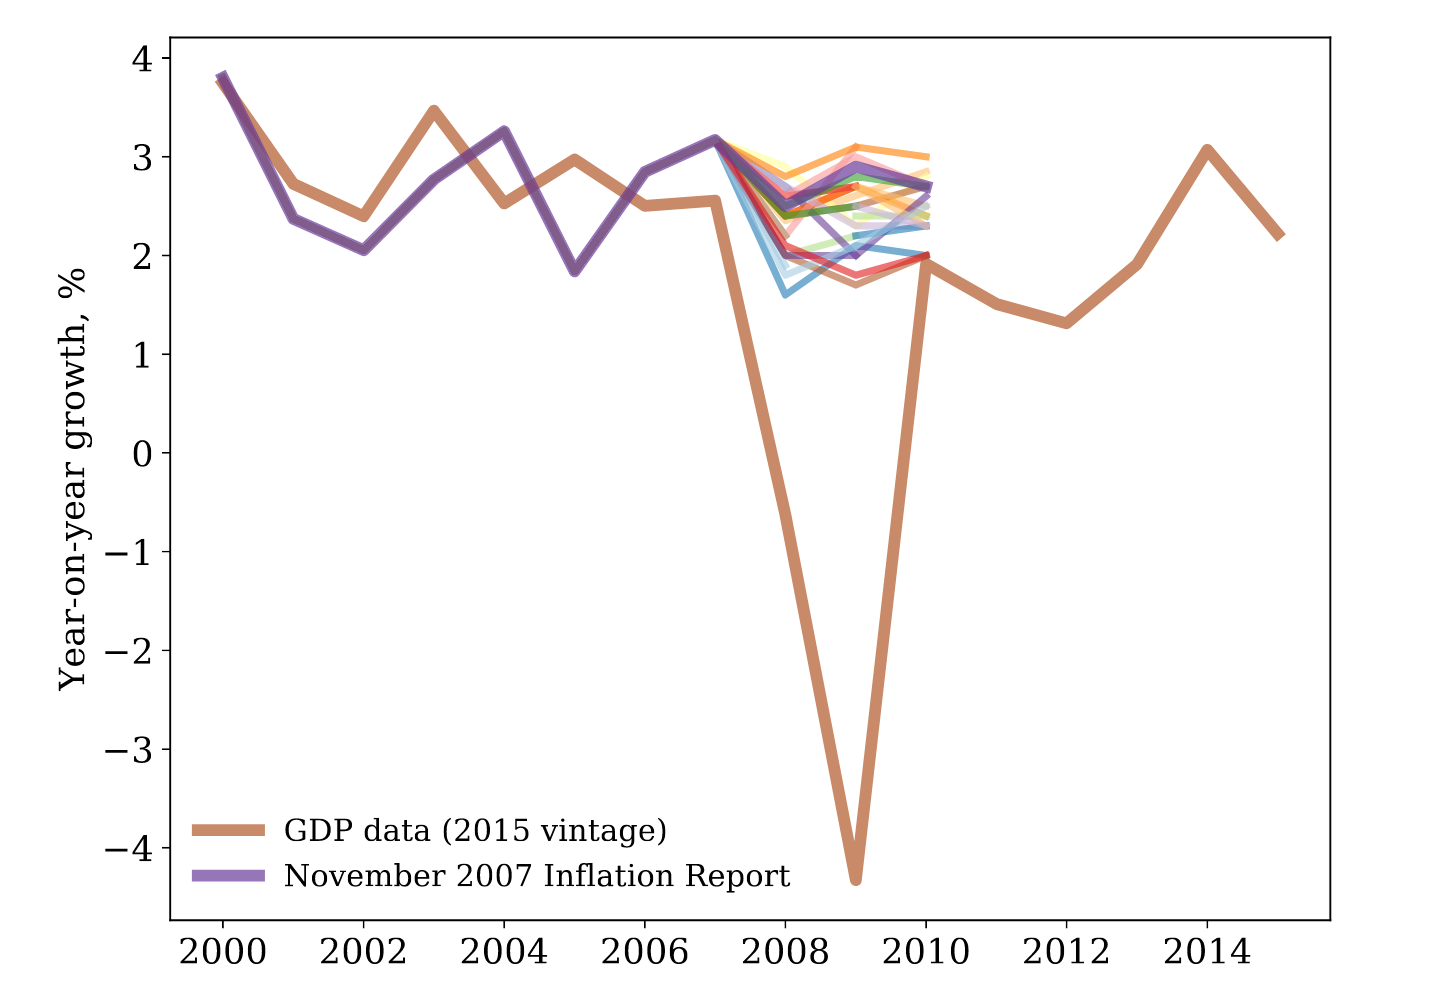
\includegraphics[width=0.8\textwidth]{Images/Forecast_Comparison.png}
        \caption{Many models failed to predict the Financial Crisis of 2008. Source: \cite{haldane_interdisciplinary_2018}.}
        \label{fig:forecast-comparison}
    \end{figure}
\end{frame}

\begin{frame}{What are the typical elements of an agent-based model?}
    \begin{columns}
\begin{column}{0.5\textwidth}
     \begin{itemize}
        \item \textbf{Local} and/or \textbf{global} interaction with other agents or the environment.
        \item Decision-making via simple \textbf{heuristics}.
        \item \textbf{Non-rational} (typically adaptive) expectations.
        \item Interaction structured by \textbf{topology or network}.
        \item An environment in which agents act and react.
        \item Global dynamics are \textbf{emergent} from local interactions.
    \end{itemize}
\end{column}
\begin{column}{0.5\textwidth}
        \begin{figure}
        \centering
    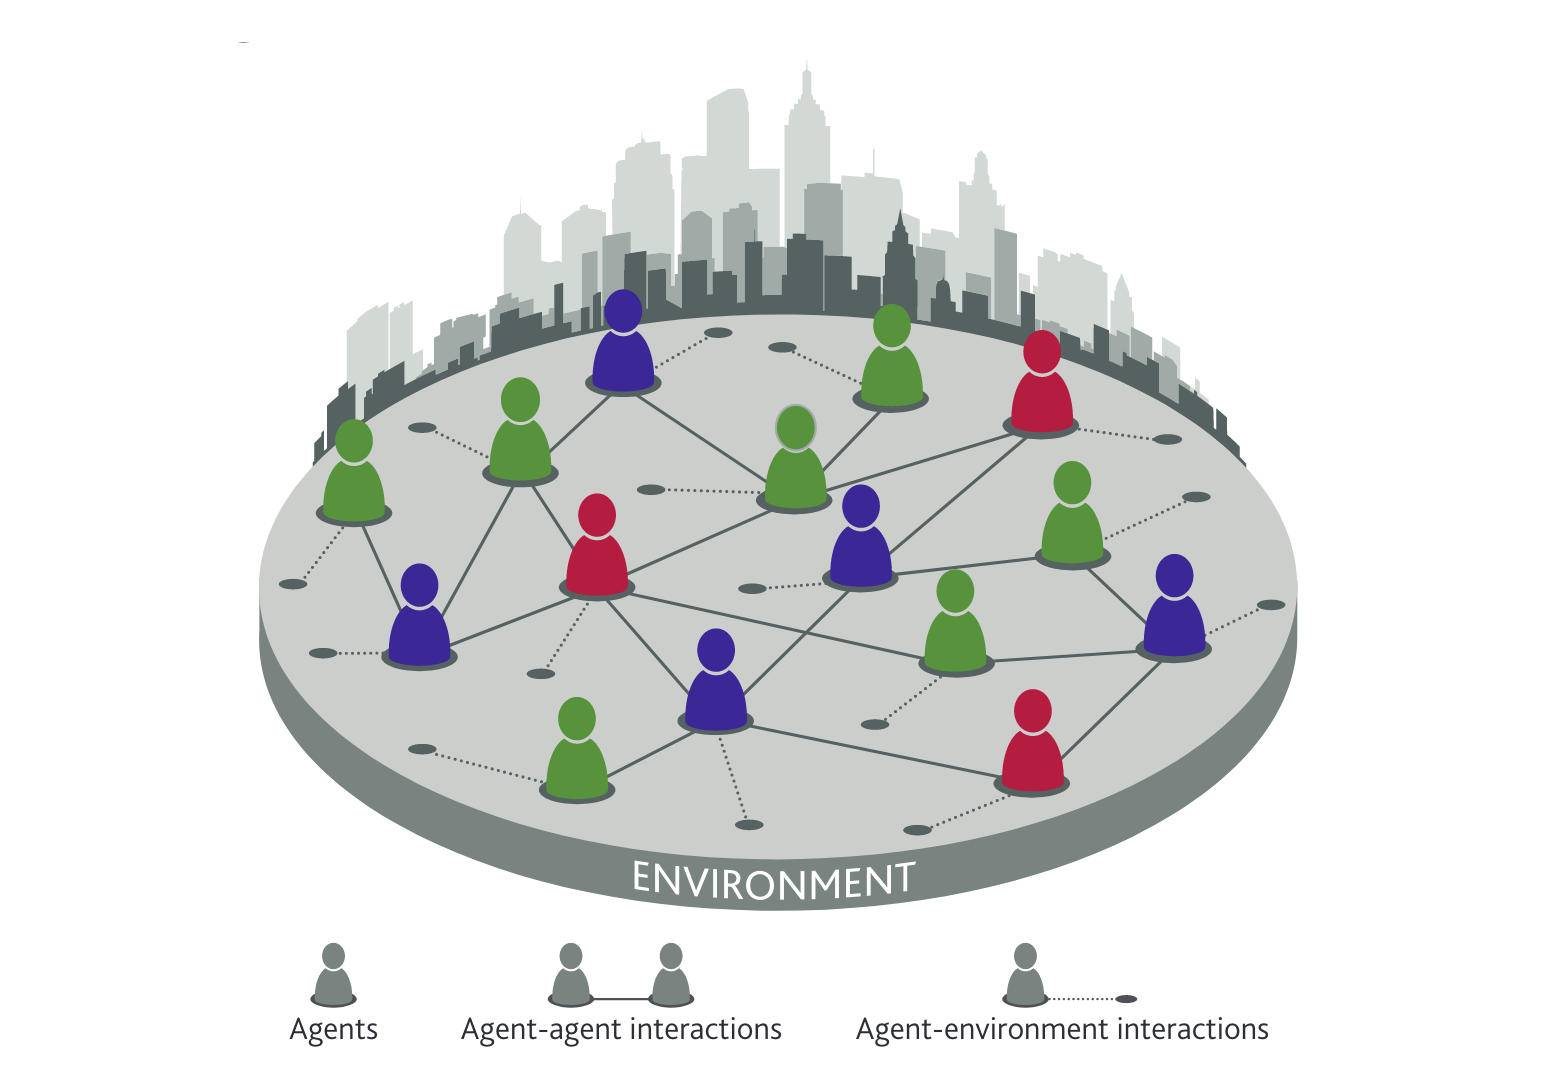
\includegraphics[width=\textwidth]{Images/ABMScheme.png}
        \caption{A schematic of the elements of an agent-based model and their interactions. Source: \cite{haldane_interdisciplinary_2018}.}
        \label{fig:abm-schematic}
    \end{figure}
\end{column}
\end{columns}
\end{frame}

\begin{frame}{Classic example: the segregation model of \cite{schelling_models_1969}}
\begin{columns}
\begin{column}{0.65\textwidth}
\begin{itemize}
        \item \textbf{Agent}: household / person.
        \item \textbf{State}: happiness of the agent: the fraction $B$ of the neighbourhood that is the same type.
        \item \textbf{Action}: if the fraction $B \leq B_a$, move to an empty spot.
        \item \textbf{Topology}: agents interact only with their direct neighbours.
        \item \textbf{Environment}: the rectangular grid on which the agents live.
        \item Segregation is a \textbf{global phenomenon that emerges from local interactions}, already for mild preferences ($B_a \geq 0.3$).
   \end{itemize}
\end{column}
\begin{column}{0.35\textwidth}
    \begin{figure}
        \centering
        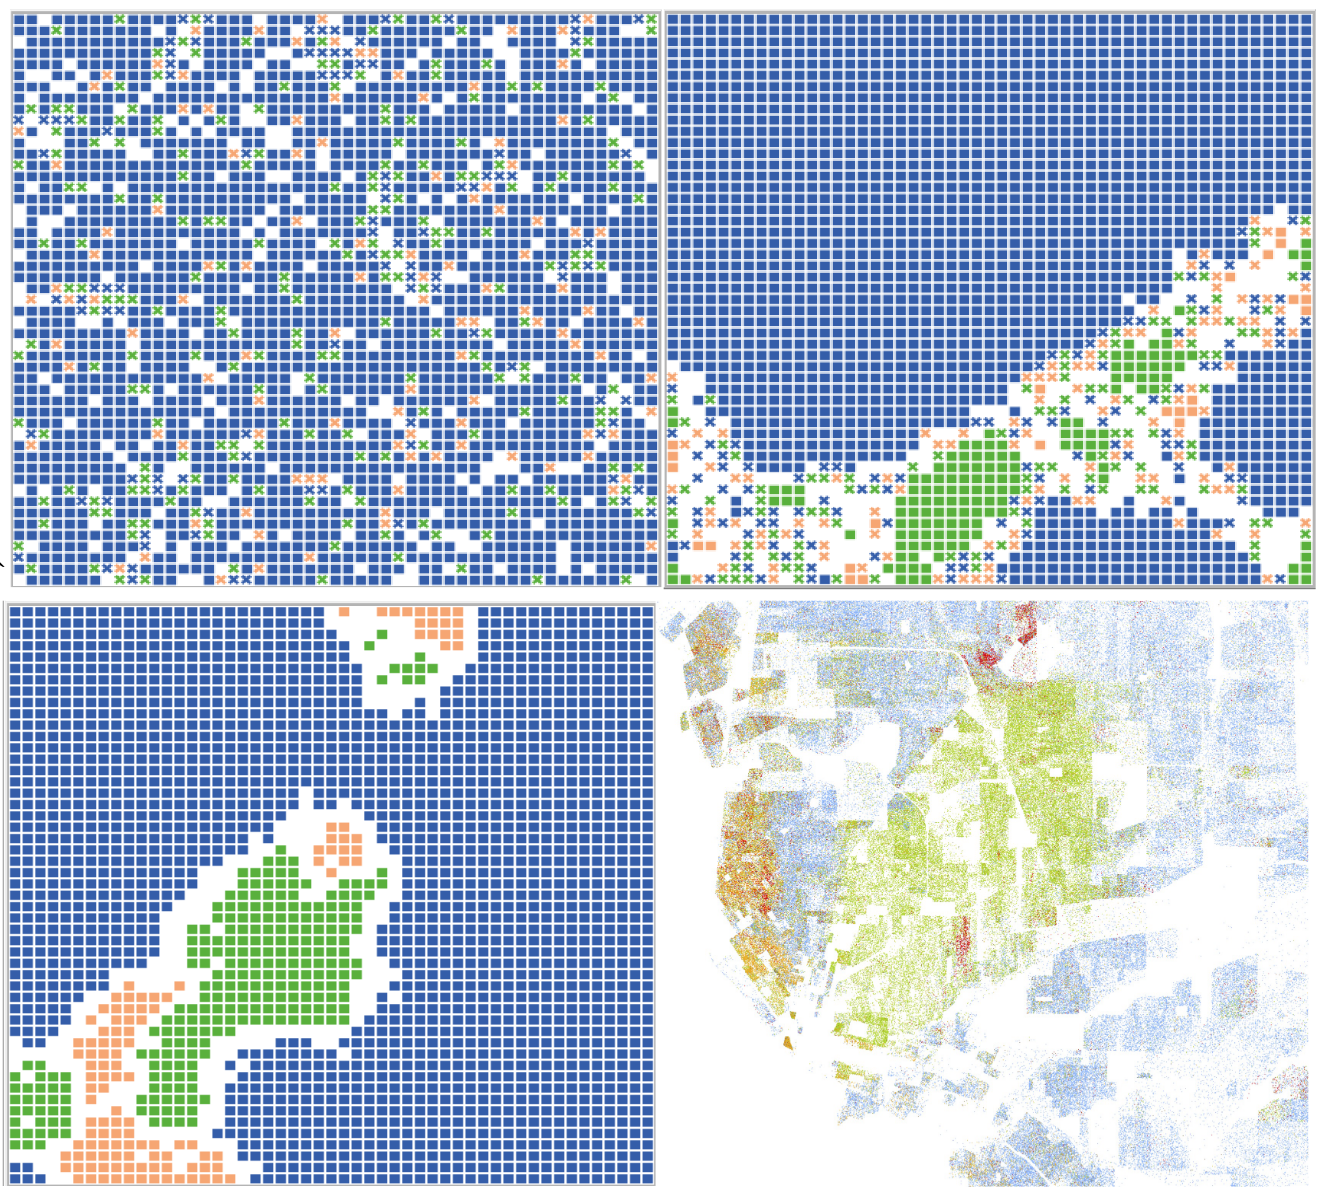
\includegraphics[width=\textwidth]{figs/Schelling.png}
        \caption{One of the first economic agent-based models \citep{schelling_models_1969}. Source: \cite{axtell_agent-based_nodate}.}
        \label{fig:schelling}
    \end{figure}
\end{column}
\end{columns}
\end{frame}

\begin{frame}{From qualitative to quantitative ABMs}
    \begin{itemize}
        \item \textbf{Qualitative} macro ABMs (e.g.\ \cite{assenza_emergent_2015}) generate emergent business cycles from agent interactions, but are validated only against \emph{stylised facts}.
        \item \textbf{Quantitative} ABMs need not be large: \emph{stylised} models with few parameters, such as the \cite{brock_heterogeneous_1998} heterogeneous-agent asset-pricing model, can be \emph{estimated} directly on data (our benchmark in the calibration section).
        \item Today we focus on a \textbf{large-scale, data-driven} ABM: the \cite{poledna_economic_2019} model, calibrated directly to national-accounts data and validated by \emph{out-of-sample forecasting}.
        \item We then discuss advanced calibration techniques for the remaining free parameters, and an application to the wage--price spiral.
    \end{itemize}
\end{frame}

\section{Poledna et al. model}

\begin{frame}{Model overview}
    \begin{itemize}
        \item  All economic activities classified by the \textbf{European System of Accounts} (ESA 2010).
        \item  \textbf{Complete GDP identity} via the production, income, and expenditure approaches simultaneously.
        \item  \textbf{Adaptive learning} instead of rational expectations.
        \item \textbf{Decentralized markets} via search-and-matching with \textbf{trade frictions}.
        \item \textbf{Multi-sector production network} calibrated from input-output tables.
        \item \textbf{Stock-flow consistent} accounting across all sectors.
        \item \textbf{Non-linear amplification} of shocks generates \textbf{endogenous crises} without requiring large exogenous disturbances.
    \end{itemize}
\end{frame}

\begin{frame}{Model overview: flow diagram}
    \begin{figure}
        \centering
        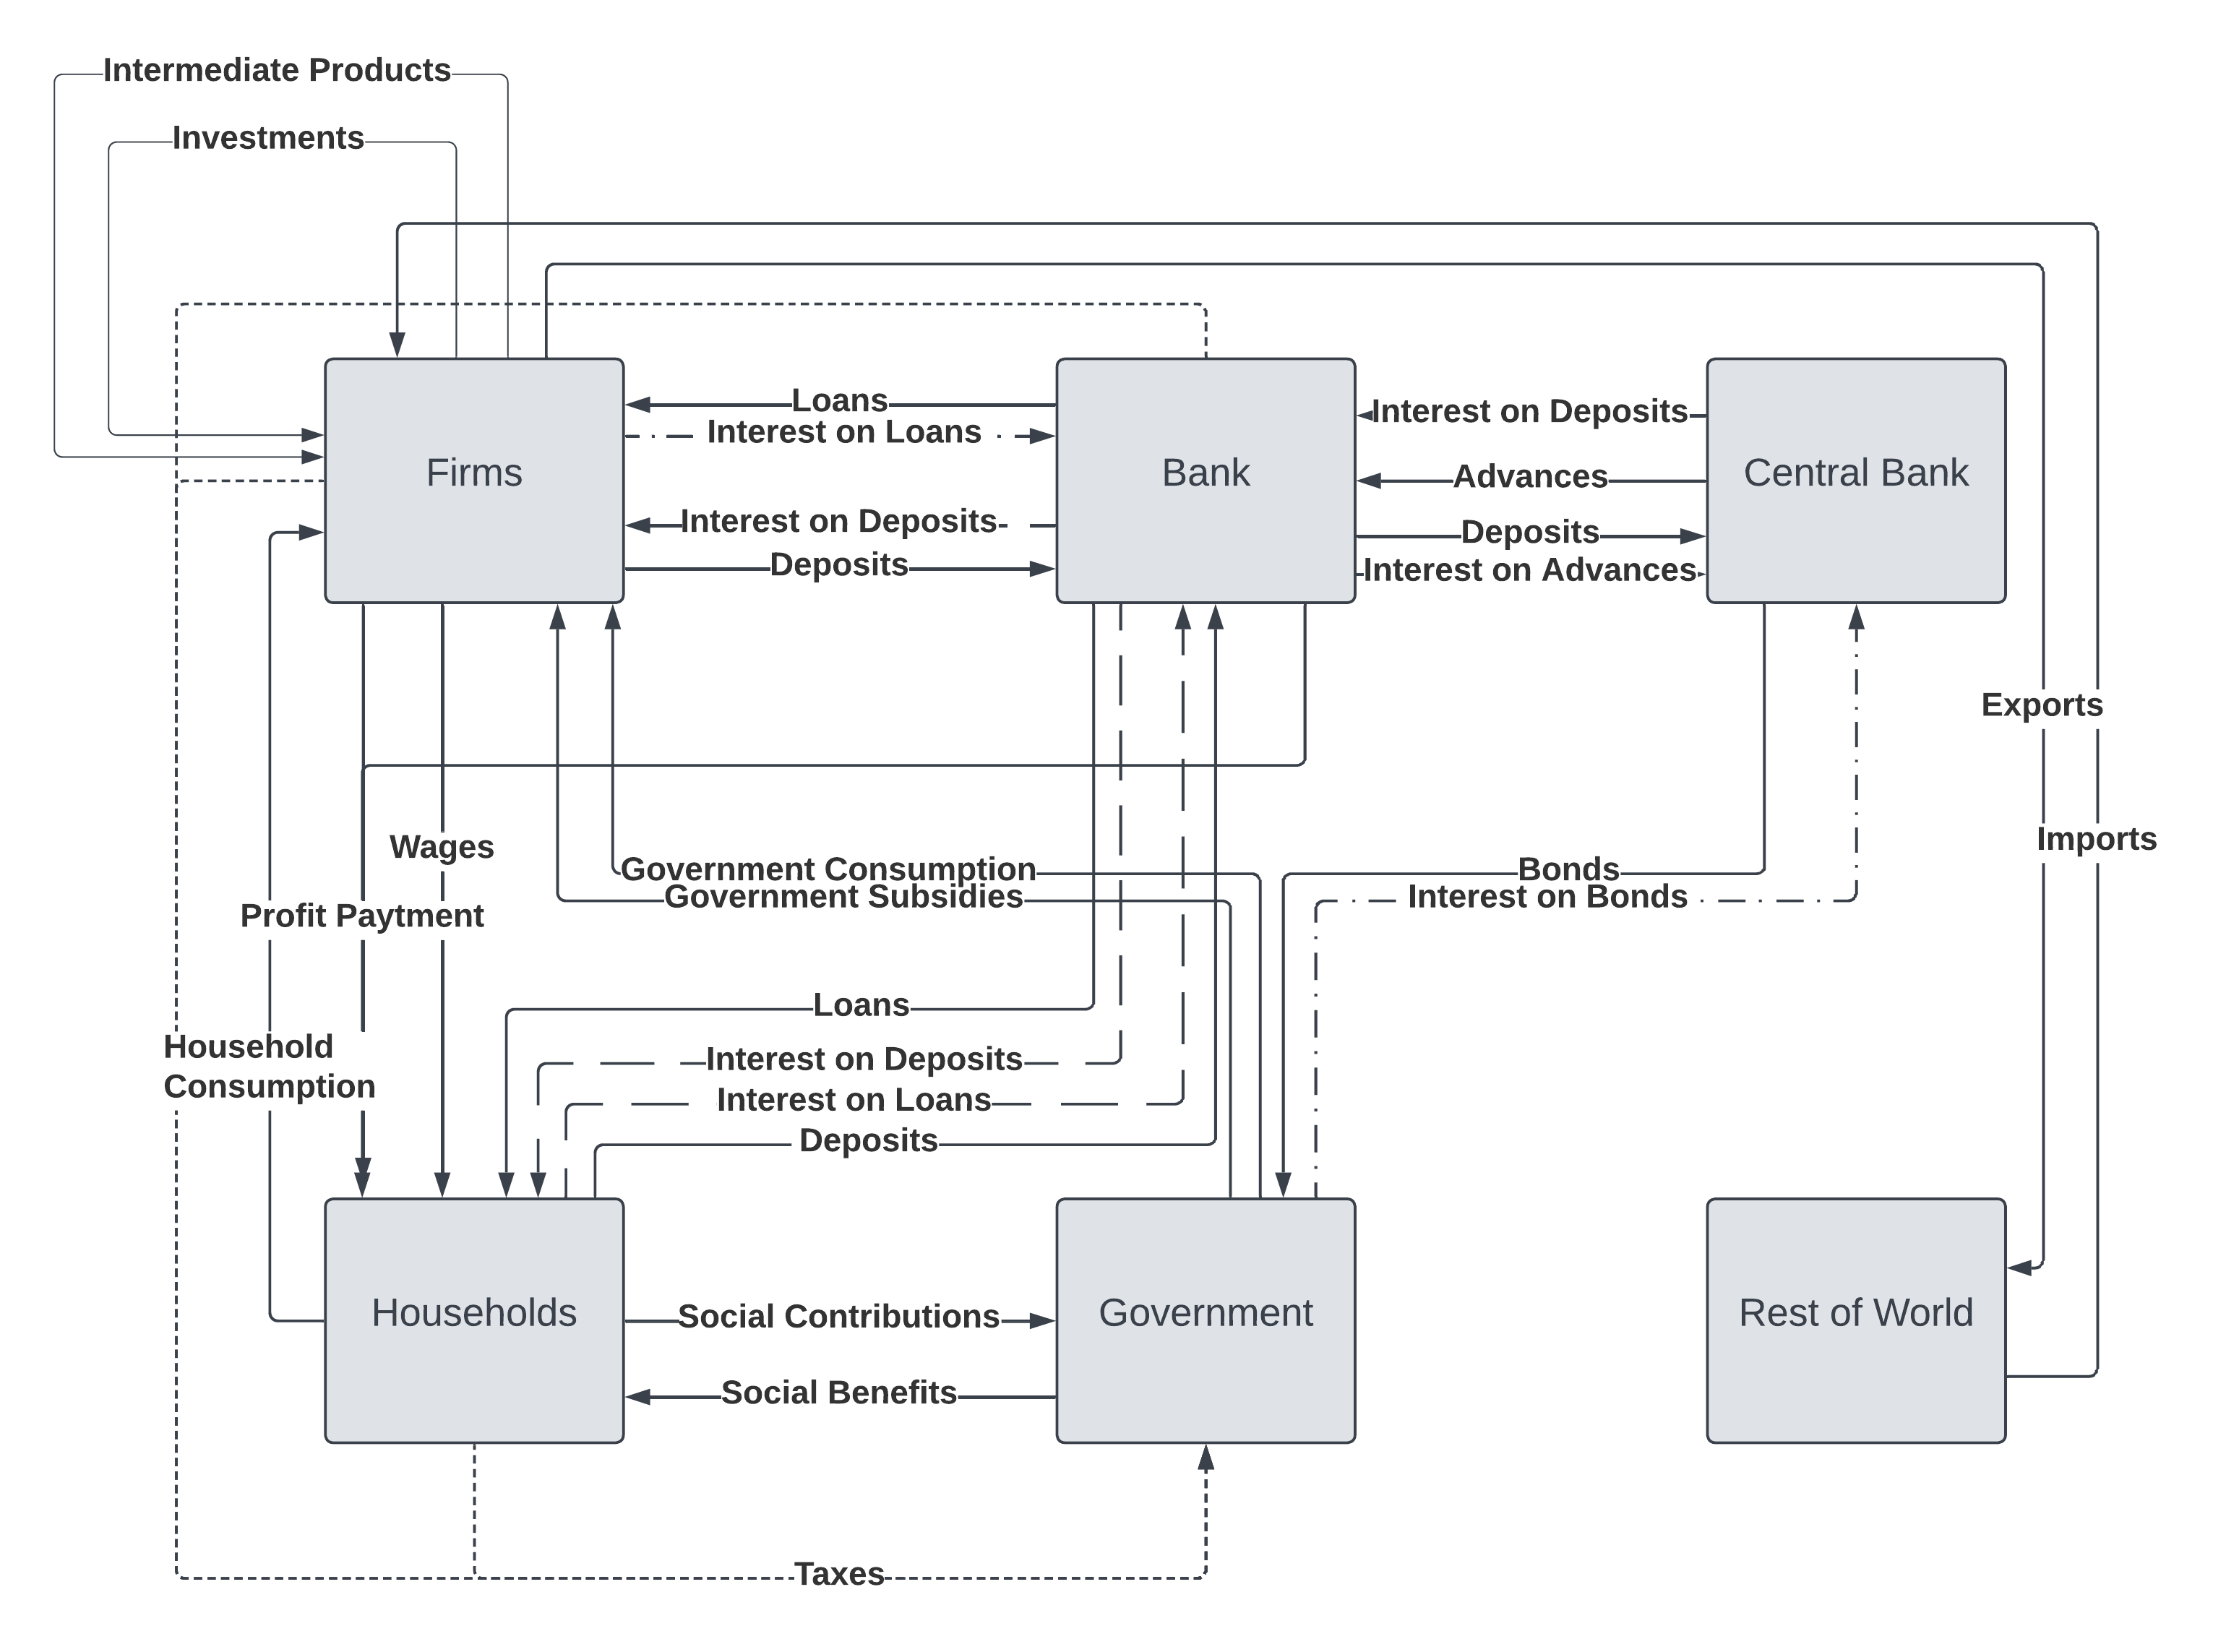
\includegraphics[width=0.85\textwidth]{figs/Diagram_poledna}
        \caption{Flow diagram of the model. }
        \label{fig:model-flow-diagram}
    \end{figure}
\end{frame}

\begin{frame}{Household behaviour: consumption, savings, expectations}
    \textbf{Consumption, Savings \& Expectations:}
    \begin{itemize}\setlength\itemsep{0.1em}
        \item Expected income depends on activity status and expectations.
        \item Consumption budget: $C^d_h(t) = \frac{\psi Y^e_h(t)}{1 + \tau^{VAT}}$ where $\psi \in (0,1)$ is propensity to consume
        \item Budget allocation: $C^d_{hg}(t) = \frac{b^{HH}_g P_g(t-1)}{P^{HH}(t-1)}C^d_h(t)$ where $b^{HH}_g$ is consumption coefficient
        \item $D_h(t) = D_h(t-1) + Y_h(t) - (1+\tau^{VAT})C_h(t) - (1+\tau^{CF})I_h(t) + \text{interest}$
        \item Expectations: agents use optimal AR(1) forecasting rules updated each period via OLS,
        \begin{align*}
        \mathbb{E}^*_t[\pi_{t+1}] = \alpha^\pi_t \pi_t + \beta^\pi_t, \quad
        \mathbb{E}^*_t[y_{t+1}] = \alpha^y_t\, y_t + \beta^y_t.
        \end{align*}
    \end{itemize}
\end{frame}

\begin{frame}{Household heterogeneity: four types}
    \begin{columns}
    \begin{column}{0.55\textwidth}
    \begin{itemize}\setlength\itemsep{0.3em}
        \item \textbf{Employed} ($H^{\mathrm{E}}_t$): supply labour to a specific sector, earn sector-specific wage $w_{i,t}$.
        \item \textbf{Unemployed} ($H^{\mathrm{U}}_t$): involuntarily idle, receive benefits $\theta^{\mathrm{UB}} w_{h,t}$.
        \item \textbf{Investor}: one per firm, owns firm equity, receives dividends $\theta^{\mathrm{DIV}}(1-\tau^{\mathrm{FIRM}})\Pi_{i,t}$.
        \item \textbf{Inactive} ($H^{\mathrm{inact}}$): outside the labour force, receive social transfers $sb^{\mathrm{inact}}_t$.
    \end{itemize}
    \end{column}
    \begin{column}{0.45\textwidth}
    \footnotesize
    \textbf{Common to all households:}
    \begin{itemize}
        \item same MPC $\psi $
        \item invest fraction $\psi^{\mathrm{H}}$ of income in dwellings
        \item purchase consumption via goods-market S\&M
    \end{itemize}
    \vspace{0.3em}
    Heterogeneity is what lets the model track \textbf{distributional effects} through the income and capital accounts.
    \end{column}
    \end{columns}
\end{frame}

\begin{frame}{Firms}
    \begin{itemize}
        \item Firms produce output using labour, intermediate inputs and raw material, and capital using a \textbf{Leontief} production function $Y_{i,t}=\min \left(Q_{i,t}^{\mathrm{S}}, \beta_i M_{i,t}, \alpha_{i,t} N_{i,t}, \kappa_i K_{i,t-1}\right).$
        \item Firms face demand via the \textbf{decentralized markets}.
        \item Firms set quantity and price based on \textbf{boundedly rational expectations} of \textbf{growth and inflation}.
        \item Firms can finance expenditures by \textbf{borrowing} from the bank.
        \item Firms can become \textbf{bankrupt} if they are both insolvent and have negative equity value.
    \end{itemize}
\end{frame}

\begin{frame}{Firm quantity and price setting}
    \begin{itemize}
        \item Firms are boundedly rational: they do not know their equilibrium position, so they set \textbf{supply} and \textbf{price} on AR(1) expectations of growth and inflation.
        \item \textbf{Quantity}: scale last period's demand by expected aggregate growth $\gamma^{\mathrm{e}}_t$,
        \[ Q^{\mathrm{s}}_{i,t} = Q^{\mathrm{d}}_{i,t-1}\,(1+\gamma^{\mathrm{e}}_t), \]
        with $\gamma^{\mathrm{e}}_t$ from an AR(1) (or VAR(1)) on aggregate output.
        \item \textbf{Price}: previous price scaled by \textbf{cost-push} and \textbf{expected (built-in)} inflation,
        \[ P_{i,t} = P_{i,t-1}\,\underbrace{(1+\pi^{\mathrm{c}}_{i,t})}_{\text{cost-push}}\,\underbrace{(1+\pi^{\mathrm{e}}_t)}_{\text{built-in}}, \]
        where $\pi^{\mathrm{c}}_{i,t}$ aggregates the change in unit \textbf{labour}, \textbf{intermediate} and \textbf{capital} costs (plus net product/production taxes and a target operating margin).
    \end{itemize}
\end{frame}

\begin{frame}{Goods market: search and matching}
    \begin{itemize}
        \item No Walrasian auctioneer: each period buyers (households, government, firms purchasing inputs/capital) \textbf{visit randomly chosen firms} and buy from the cheapest available, forming a buyer--seller network.
        \item A firm $i$ is drawn by weighted sampling: more likely if it charges a \textbf{low price} and is \textbf{large}:
    \end{itemize}
    \vspace{-0.3em}
    \[
    pr^{\text{price}}_{i,t} = \frac{e^{-2 P_{i,t}}}{\sum_{i\in I_{s=g}} e^{-2 P_{i,t}}}, \quad
    pr^{\text{size}}_{i,t} = \frac{Y_{i,t}}{\sum_{i\in I_{s=g}} Y_{i,t}}, \quad
    pr^{\text{cum}}_{i,t} = \frac{pr^{\text{price}}_{i,t} + pr^{\text{size}}_{i,t}}{2}.
    \]
    \vspace{-0.3em}
    \begin{itemize}
        \item Realized \textbf{sales} are capped by production plus inventory:
        $Q_{i,t} = \min\!\left(S_{i,t-1} + Y_{i,t},\, Q^{\mathrm{d}}_{i,t}\right)$.
        \item Demand that cannot be met $\Rightarrow$ \textbf{involuntary saving}; output left unsold $\Rightarrow$ \textbf{inventory} $\Delta S_{i,t} = Y_{i,t} - Q_{i,t}$.
    \end{itemize}
\end{frame}

\begin{frame}{Labour market: search and matching}
    \begin{itemize}
        \item The labour market is solved \textbf{before} the goods market each quarter.
        \item Firms post vacancies consistent with their expected production and the Leontief labour coefficient:
        $N^{\mathrm{d}}_{i,t} = Q^{\mathrm{s}}_{i,t}/\alpha_{i,t}$.
        \item Unemployed households apply to firms in random order; matching probability is weighted by \textbf{firm size} and \textbf{posted wage}.
        \item Hiring/firing is frictional: if $N^{\mathrm{d}}_{i,t} < N_{i,t-1}$ firms lay off the excess; if $N^{\mathrm{d}}_{i,t} > N_{i,t-1}$ they hire from the unemployed pool.
        \item Wages update slowly around the sector-specific average $\bar{w}_i$, indexed to expected inflation.
    \end{itemize}
\end{frame}

\begin{frame}{Input-output network}
\begin{figure}
    \centering
    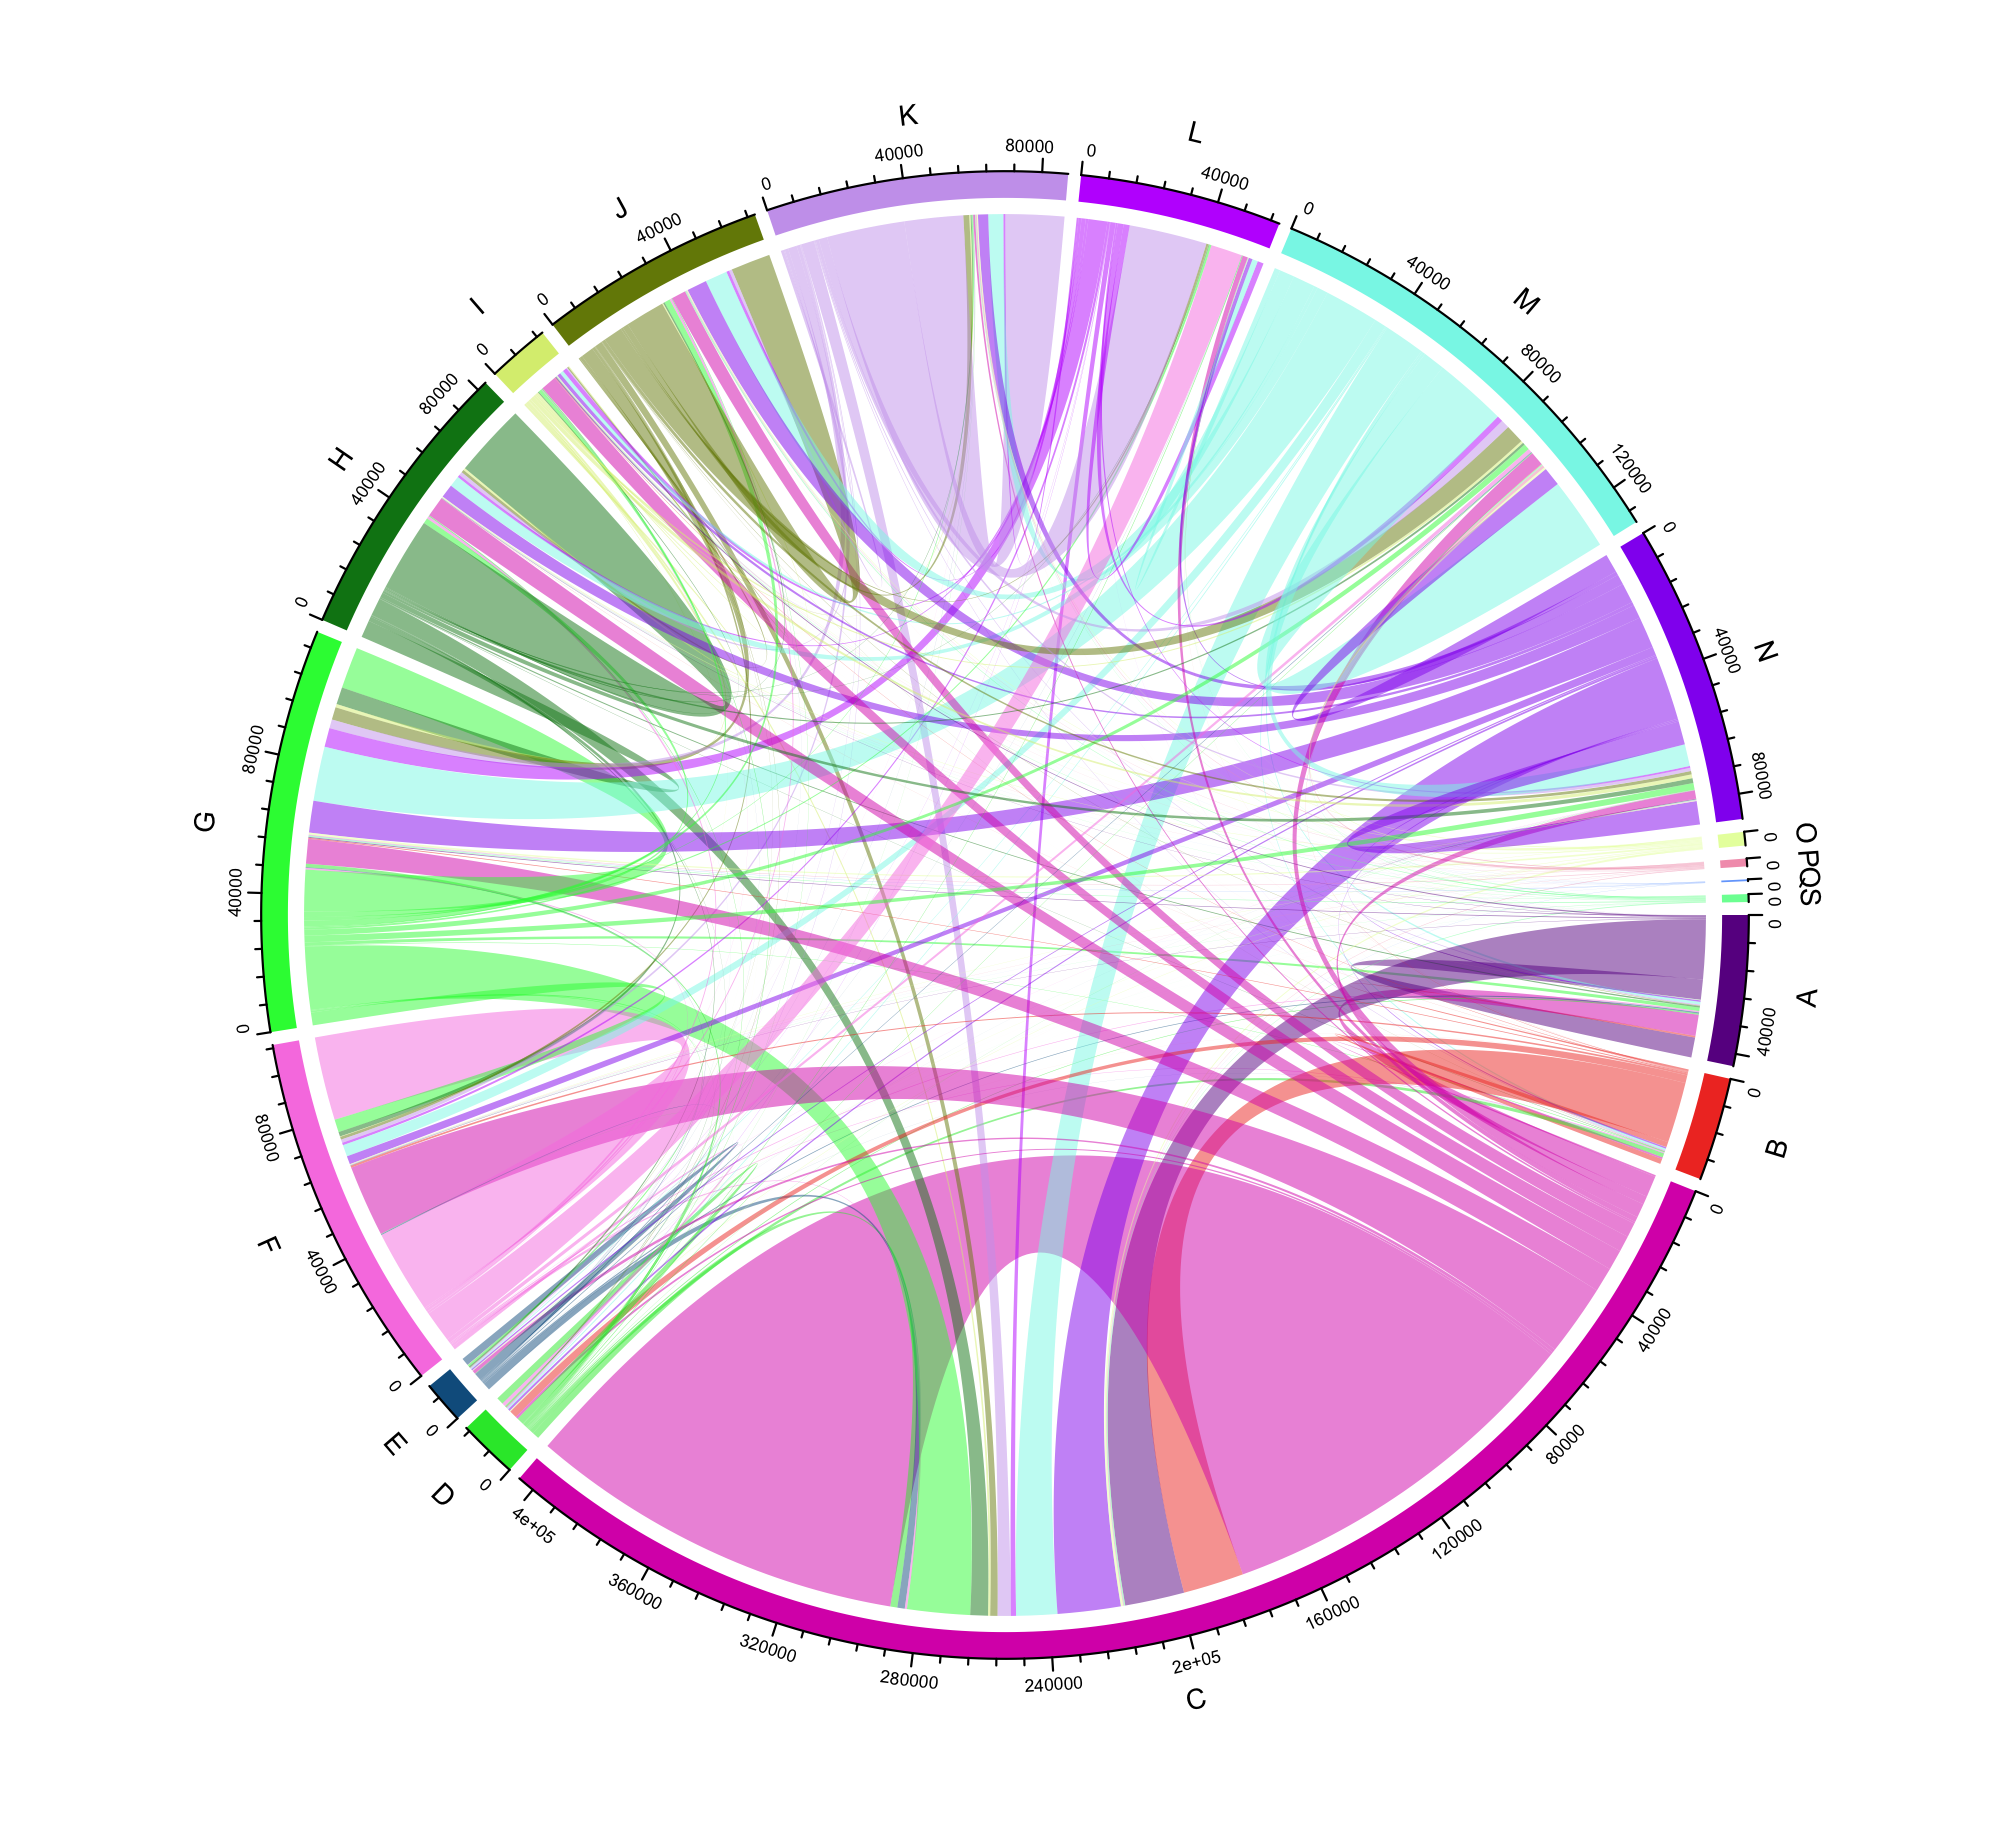
\includegraphics[trim = 3cm 3cm 3cm 3cm, clip, width = 0.6\textwidth]{figs/Rplot03.png}
    \captionsetup{singlelinecheck=off}
    \caption[foo bar]{Intermediate consumption between 19 industries derived from Eurostat input-output table.}
    \label{fig:IO}
\end{figure}
\end{frame}

\begin{frame}{Remainder of model}
    \label{ReturnOverview}
    \begin{itemize}
        \item \textbf{Government} consumes on the goods market, levies taxes, pays out transfers and social benefits.
        \item \textbf{Banking sector} provides loans to firms subject to a minimum capital requirement and a risk assessment; holds household and firm deposits.
        \item \textbf{Central bank} sets the policy rate via a Taylor rule and holds government debt as an asset.
        \item \textbf{Rest of the world} exports to and imports from the domestic economy via the decentralized markets.
    \end{itemize}
\end{frame}

\begin{frame}{Fiscal and monetary closure}
    \begin{columns}[T]
    \column{0.5\textwidth}
    \textbf{Government (fiscal)}
    \begin{itemize}\footnotesize
        \item \textbf{Revenue}: income tax, VAT, corporate tax, social contributions (employer, employee), capital-formation tax, export tax, sector-specific production/product taxes.
        \item \textbf{Spending}: government consumption, unemployment benefits at replacement rate, inactive transfers, interest on debt.
        \item \textbf{Debt dynamics}:
        \begin{equation*}\footnotesize
            L^{\mathrm{G}}_t = L^{\mathrm{G}}_{t-1} + (\text{expenditures}_t - \text{revenues}_t)
        \end{equation*}
    \end{itemize}

    \column{0.5\textwidth}
    \textbf{Bank \& central bank (monetary)}
    \begin{itemize}\footnotesize
        \item \textbf{Basel III capital requirement}:
        $E_{k,t}/\sum_i L_{i,t} \geq \zeta = 3\%$. When bad-debt write-offs shrink bank equity $E_{k,t}$, the constraint binds and credit to \emph{other} firms is rationed, this is the credit channel of the bankruptcy cascade.
        \item \textbf{Loan-to-value} on new loans: $L_i/(\bar{P}^{\mathrm{CF}} K_i) \leq \zeta^{\mathrm{LTV}} = 60\%$.
        \item \textbf{Loan rate}: $r_t = \bar{r}_t + \mu$, fixed markup $\mu = 2.9\%$ over the policy rate.
        \item \textbf{Policy rate} $\bar{r}_t$: generalised Taylor rule reacting to \emph{euro-area} inflation and growth.
    \end{itemize}
    \end{columns}
    \vspace{0.4em}
    \footnotesize
    Every tax, transfer, loan, and interest payment is recorded inside the SFC structure: the government and banking sectors are \emph{part of} the balance-sheet closure, not black boxes bolted on.
\end{frame}

\begin{frame}{Sequence of events in each quarter}
    \small
    Each period $t$ is one quarter. The model is solved recursively:
    \begin{enumerate}
        \item[\textbf{(i)}] \textbf{Expectations}: agents OLS-update their AR(1) rules for output and inflation using last period's realisation.
        \item[\textbf{(ii)}] \textbf{Exogenous shocks}: draw from the AR(1) processes for exports, imports, government consumption, euro-area growth, euro-area inflation.
        \item[\textbf{(iii)}] \textbf{Credit and labour markets}: search-and-matching solved. Firms apply for loans and hire/fire; unemployed households seek jobs.
        \item[\textbf{(iv)}] \textbf{Goods market}: search-and-matching solved. Households, firms (intermediate inputs), government, and foreign consumers meet firms; production and sales happen.
        \item[\textbf{(v)}] \textbf{Accounting}: update all stock and flow variables; check insolvencies; compute profits, taxes, transfers.
    \end{enumerate}
    \vspace{0.3em}
    Each reference quarter is simulated \textbf{500 times} (Monte Carlo); the forecast is the average across runs.
\end{frame}

\section{Calibration}
\begin{frame}{Data Sources}
    \begin{itemize}
        \item Eurostat national accounts data
        \item Census and business demography data
        \item Input-output tables
        \item Government statistics and sector accounts
        \item Statutory guidelines, financial regulation (Basel III), and banking practices
    \end{itemize}
\end{frame}

\begin{frame}{How big is the model?}
    \begin{columns}
    \begin{column}{0.5\textwidth}
    \textbf{Agent counts (Austria, 2010:Q4)}
    \footnotesize
    \begin{tabular}{lr}
        \toprule
        Economically active persons & 4{,}729{,}215 \\
        Inactive persons            & 4{,}130{,}385 \\
        Firms / investors\footnotemark & $\approx\,$611{,}280 \\
        Government entities         & 152{,}820 \\
        Foreign consumers           & 305{,}639 \\
        Foreign firms (imports)     & $\approx 50$ \\
        \bottomrule
    \end{tabular}
    \normalsize
    \vspace{0.5em}

    \textbf{Total: $\sim 9.9$ million heterogeneous agents.}
    \footnotetext{\tiny Derived from the paper's Table 2: $J = 25\%$ of domestic firms, $L = 50\%$; both give $\approx 611{,}280$.}
    \end{column}
    \begin{column}{0.5\textwidth}
    \textbf{Sector structure}
    \begin{itemize}\footnotesize
        \item \textbf{64 NACE industries} (the I-O figure earlier showed an aggregated 19 for visual clarity)
        \item Firm size distribution within each industry follows a \textbf{power law}, calibrated from Eurostat business demography
        \item Industry-specific: productivities $\bar{\alpha}_i, \kappa_i, \beta_i$, depreciation $\delta_i$, wages $\bar{w}_i$
        \item No representative firm, no representative consumer
    \end{itemize}
    \end{column}
    \end{columns}
\end{frame}

\begin{frame}{Data-based initialisation \& no burn-in}
    \textbf{Why the Poledna model needs no burn-in:}
    \vspace{0.6em}
    \begin{enumerate}
        \item[\textbf{1.}] \textbf{SFC accounting matches ESA\,2010.} The model's sectoral accounting \emph{is} the national accounts framework. At $t{=}0$, balance sheets and flows are loaded directly from Austrian Eurostat data.

        \vspace{0.3em}
        \item[\textbf{2.}] \textbf{The initialisation is a quasi-fixed point.}. If we supress the growth processes, the model fluctuates around it's initial conditions.

        \vspace{0.3em}
        \item[\textbf{3.}] \textbf{Contrast with standard ABMs.} Most agent-based models start from an arbitrary or stylised initial state that is \emph{not} a rest point of the dynamics. Even without shocks, the model must first converge to an attractor. 
    \end{enumerate}
    \vspace{0.4em}
    \footnotesize
    \emph{Caveat:} the AR(1) expectation parameters and five exogenous shock processes are still estimated on pre-sample data (1997\,:\,Q1--). There is no dynamic burn-in, but there is a historical estimation window.
\end{frame}

\begin{frame}{Calibration Process}
    \begin{itemize}
        \item The biggest innovation of the model is that almost all parameters are directly identified from Eurostat national accounts.
        \item At time $t = 0$, the initial values of the model match the data found in the national accounts (or are imputed from the same data at the micro level).
        \item Combined with stock-flow consistency, this means no dynamic burn-in is required (see earlier slide).
        \item The parameters are identified using the datasets listed on the previous slide.
        \item For example, the marginal propensity to consume $\psi$ is calibrated as the ratio of household consumption to disposable income.
        \item A small number of parameters still may be inferred. More on this later.
    \end{itemize}
\end{frame}

\begin{frame}{The full parameter set: (almost) no free parameters}
    \footnotesize
    \begin{tabular}{@{}lll@{}}
        \toprule
        \textbf{Source} & \textbf{Example parameters} & \textbf{Value} \\
        \midrule
        \multirow{2}{*}{Census / business demography}
            & Active persons $H^{\mathrm{act}}$ & 4{,}729{,}215 \\
            & Firms per industry $I_s$          & power law \\
        \midrule
        \multirow{3}{*}{Input--output tables}
            & Technology coefs $a_{sg}$          & matrix \\
            & Labour productivity $\bar{\alpha}_i$ & industry \\
            & Consumption coefs $b^{\mathrm{HH}}_g$ & by product \\
        \midrule
        \multirow{5}{*}{Gov.\ statistics / sector accounts}
            & Income tax $\tau^{\mathrm{INC}}$       & 0.2134 \\
            & VAT $\tau^{\mathrm{VAT}}$              & 0.1529 \\
            & Corporate tax $\tau^{\mathrm{FIRM}}$   & 0.0762 \\
            & MPC $\psi$                             & 0.9394 \\
            & Dividend payout $\theta^{\mathrm{DIV}}$ & 0.7768 \\
        \midrule
        \multirow{4}{*}{Basel III / statutes}
            & Capital ratio $\zeta$                  & 0.03 \\
            & LTV $\zeta^{\mathrm{LTV}}$             & 0.60 \\
            & Unempl.\ benefit $\theta^{\mathrm{UB}}$ & 0.3586 \\
            & Inflation target $\pi^{*}$             & 0.005 \\
        \midrule
        \multirow{3}{*}{AR(1) \& Taylor rule (estimated)}
            & Taylor smoothing $\rho$                & 0.9263 \\
            & Inflation weight $\xi^{\pi}$           & 0.3214 \\
            & Growth weight $\xi^{\gamma}$           & 1.2994 \\
        \bottomrule
    \end{tabular}
    \vspace{0.3em}

    \normalsize
    \textbf{$\sim 50$ parameters total. Only the AR(1) / Taylor-rule block is estimated; everything else is read off data or statute.}
\end{frame}



\section{External Validation}
\begin{frame}{Out-of-sample forecast performance in comparison to DSGE model}
    \centering
    \scriptsize
    \setlength{\tabcolsep}{4pt}
    \renewcommand{\arraystretch}{0.95}
    \begin{tabular}{lccccc}
        \toprule
             & GDP & Inflation & Household consumption & Investment & Euribor \\
        \midrule
        AR(1) & \multicolumn{5}{l}{\textit{RMSE-statistic for different forecast horizons}} \\
        1q   & 0.52 & 0.3  & 0.52 & 1.18 & 0.03 \\
        2q   & 0.77 & 0.28 & 0.73 & 1.78 & 0.06 \\
        4q   & 1.26 & 0.28 & 1.14 & 2.91 & 0.11 \\
        8q   & 2.12 & 0.29 & 1.93 & 4.26 & 0.16 \\
        12q  & 2.89 & 0.25 & 2.74 & 6.01 & 0.2  \\
        \midrule
        DSGE & \multicolumn{5}{l}{\textit{Percentage improvements ($+$) or losses ($-$) relative to AR(1) model}} \\
        1q   & 1.1 (0.93)    & $-$13.6 (0.05**) & 7.7 (0.25)  & $-$1.6 (0.87)  & $-$147.8 (0.00***) \\
        2q   & $-$5.7 (0.70) & $-$10.9 (0.19)   & 12.5 (0.20) & 2.4 (0.90)     & $-$183.4 (0.00***) \\
        4q   & $-$8.2 (0.76) & $-$9.6 (0.09*)   & 30.5 (0.21) & $-$10.5 (0.74) & $-$201.3 (0.00***) \\
        8q   & $-$2 (0.97)   & 2.7 (0.80)       & 38.5 (0.29) & $-$19.4 (0.57) & $-$210 (0.00***)   \\
        12q  & 3.7 (0.97)    & $-$14.9 (0.18)   & 49 (0.30)   & 0.4 (0.98)     & $-$180.4 (0.00***) \\
        \midrule
        ABM  & \multicolumn{5}{l}{\textit{Percentage improvements ($+$) or losses ($-$) relative to AR(1) model}} \\
        1q   & 1.7 (0.88)    & $-$0.2 (0.80)    & $-$16.1 (0.26) & $-$3.7 (0.12) & $-$3.6 (0.44) \\
        2q   & $-$1.8 (0.90) & $-$0.7 (0.52)    & $-$13.1 (0.56) & $-$4.3 (0.23) & $-$2.6 (0.69) \\
        4q   & $-$5.5 (0.81) & 1.5 (0.03*)      & $-$2 (0.95)    & $-$4.6 (0.26) & 2.1 (0.85)    \\
        8q   & $-$3.4 (0.97) & 1.2 (0.53)       & 11.8 (0.83)    & $-$6.9 (0.56) & 0.6 (0.98)    \\
        12q  & $-$2.7 (0.97) & 0.2 (0.80)       & 19.7 (0.79)    & $-$5.7 (0.71) & $-$0.3 (0.99) \\
        \bottomrule
    \end{tabular}

    \vspace{0.4em}
    {\tiny
    \textit{Note:} Forecast period 2010:Q2--2019:Q4. The AR(1) and the DSGE model are re-estimated each quarter. The ABM is calibrated to 39 different reference quarters. ABM results are averaged over 500 Monte Carlo simulations. $p$-values in parentheses are from (modified) Diebold--Mariano tests \citep{harveyTestingEqualityPrediction1997}, under the null that the tested model has the same accuracy as the AR(1). ${}^*$, ${}^{**}$, ${}^{***}$ denote significance at the 10, 5, and 1 per cent levels, respectively. \textit{Source:} \cite{poledna_economic_2019}, Table~4.
    }
\end{frame}

\begin{frame}{Out-of-sample forecast performance}
    \begin{figure}[!h]
	\centering
	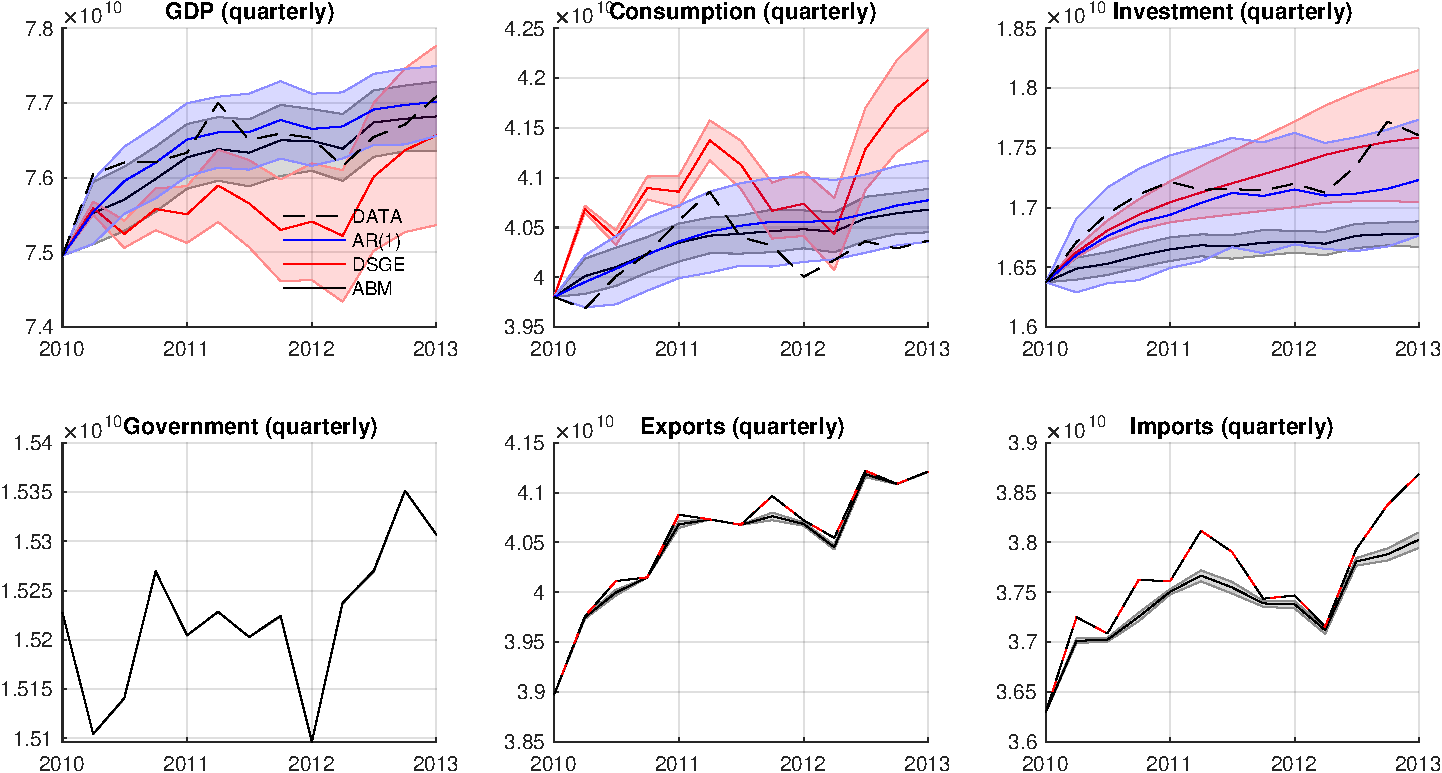
\includegraphics[width=\textwidth]{figs_Austria/out-of-sample-with-predictors_quarterly.pdf}
 \caption{\scriptsize Forecasting performance for one reference quarter (2012:Q4--2014:Q4): ABM conditional (black), DSGE conditional (red), ARX(1) (blue), and observed Eurostat data for Austria (dashed). Previous slide shows full-period RMSE (2010:Q1--2019:Q4).}
\end{figure}
\end{frame}





\begin{frame}{Quarterly out-of-sample GDP forecast decomposition}
\begin{figure}[!h]
    \centering
        \centering
        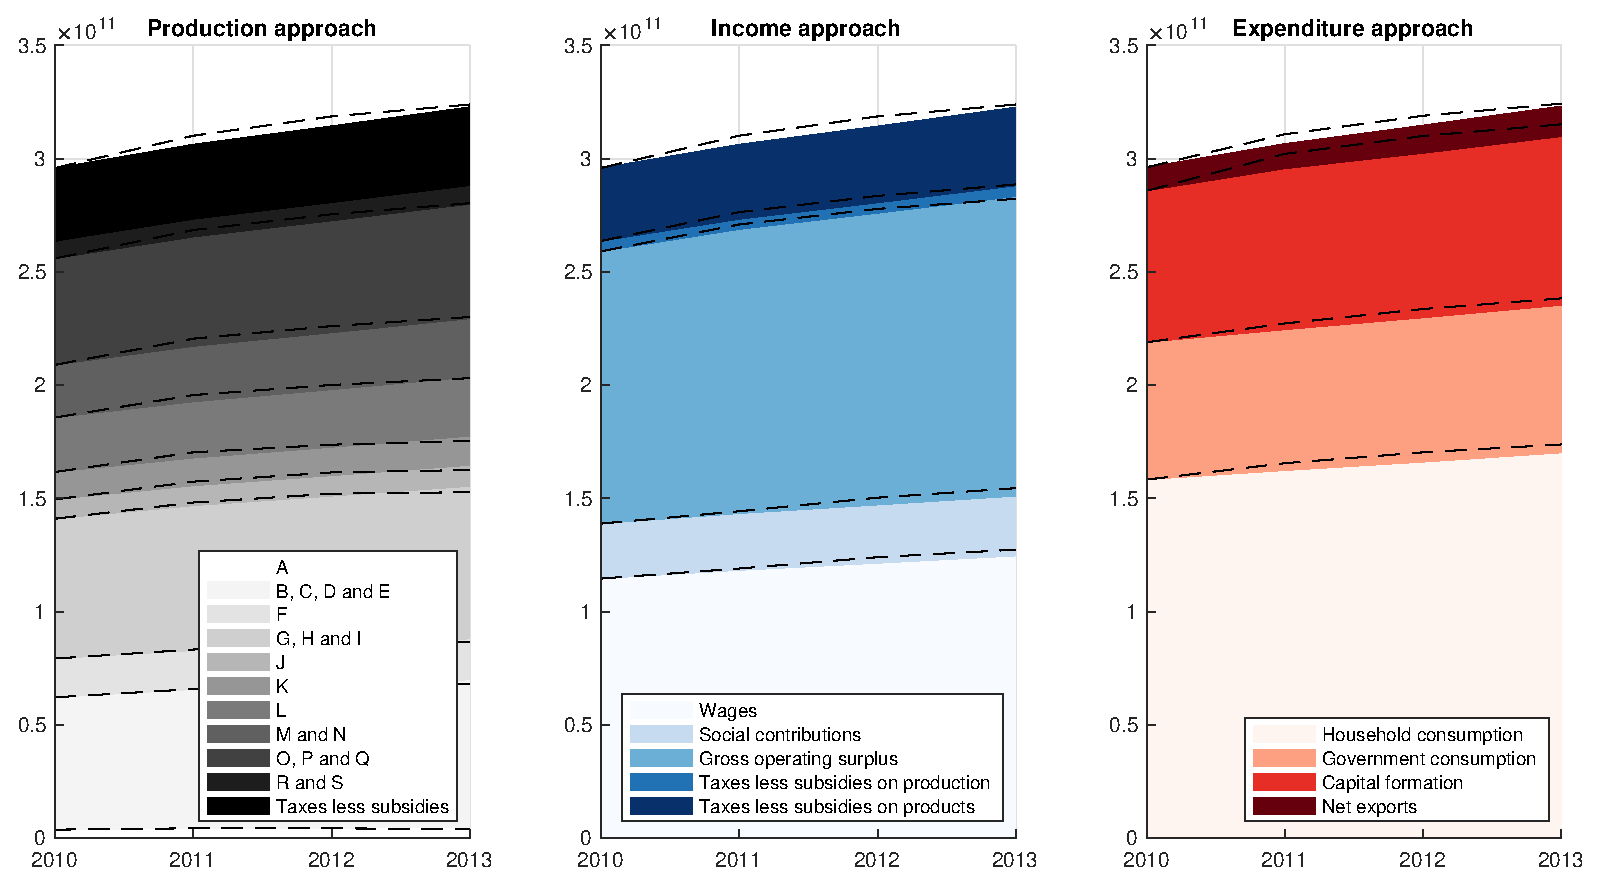
\includegraphics[width=\linewidth]{figs_Austria/national_accounting_comparison.eps}
    \caption{\footnotesize The full coloured areas are the average ABM forecast results.}
\end{figure}
\end{frame}

\begin{frame}{\cite{poledna_economic_2019} summary}
    \begin{itemize}
        \item The Poledna ABM performs \textbf{as well as or better than} the comparison models, depending on variable and horizon (not all results shown).
        \item The model is validated primarily via \textbf{out-of-sample forecasting} against observed data, in contrast to \cite{assenza_emergent_2015}, which was only validated against stylised facts.
        \item Performance improves further in a \textbf{conditional forecasting} setup where exports, imports, and government consumption are fixed at realised paths.
        \item For sectoral GVA forecasts the ABM beats the VAR in some sectors and underperforms in others (e.g.\ agriculture, real estate).
        \item A great starting point for further extensions.
        \item These models are gaining traction academically and in the policy world, e.g.\ the ECB, the Bank of England, the Bank of Canada, and the Bank of Italy.
    \end{itemize}
\end{frame}

\section{Advanced Calibration Methods}

\begin{frame}{The likelihood problem \& Neural Posterior Estimation}
\label{SBI-motivation}
    \small
    \textbf{Goal:} Bayesian inference for ABM parameters, $p(\theta \mid x_{\text{obs}}) \propto p(x_{\text{obs}}\mid\theta)\,p(\theta)$.

    \textbf{Problem:} the likelihood $p(x\mid\theta)$ is \textbf{intractable}. We can simulate $x \sim \text{ABM}(\theta)$, but cannot evaluate $p(x\mid\theta)$, so MCMC and variational inference (which need the likelihood) do not apply, and ABC suffers from the curse of dimensionality.

    \textbf{Solution: Neural Posterior Estimation} \citep{dyer_black-box_2024}:
    \begin{itemize}\setlength\itemsep{0.2em}
        \item Sample $\theta_i \sim \Phi$ (prior) and simulate $x_i \sim \text{ABM}(\theta_i)$ to build a training set $\{x_i,\theta_i\}_{i=1}^{N}$.
        \item Train a neural density estimator to approximate the posterior: $\hat{\phi} = \arg\max_\phi \sum_{i} \log q_\phi(\theta_i\mid x_i)$.
        \item \textbf{Sequential} refinement (SNPE): re-use the current posterior as the proposal for the next round of simulations (importance-reweighted to correct for the shifted proposal).
        \item Sample the posterior directly: $\theta \sim q_{\hat{\phi}}(\theta\mid x_{\text{obs}})$.
    \end{itemize}
    \textbf{Key advantage:} bypasses likelihood evaluation entirely and delivers full posterior uncertainty quantification.
\end{frame}

\begin{frame}{Does it work? SNPE vs.\ kernel density estimation}
    \begin{columns}[T]
    \begin{column}{0.5\textwidth}
    \small
    Benchmarks against KDE-based inference \citep{dyer_black-box_2024}:
    \begin{itemize}\setlength\itemsep{0.2em}
        \item \textbf{Brock--Hommes} \citep{brock_heterogeneous_1998} asset-pricing model, $\boldsymbol{\theta}=(g_2,b_2,g_3,b_3)$.
        \item Multivariate geometric Brownian motion ($d=3$).
    \end{itemize}
    \footnotesize
    \begin{tabular}{lcc}
    \toprule
                        & \textbf{KDE}      & \textbf{SNPE} \\
    \midrule
    Wasserstein (BH)    & 0.690             & \textbf{0.336} \\
    MMD (BH)            & 1.015             & \textbf{0.552} \\
    Sim.\ budget (BH)   & $1.5\times10^{5}$ & $10^{4}$ \\
    \midrule
    Wasserstein (GBM)   & 0.364             & \textbf{0.099} \\
    Sim.\ budget (GBM)  & $10^{6}$          & $10^{3}$ \\
    \bottomrule
    \end{tabular}
    \vspace{0.4em}
    \small

    \textbf{10--1000$\times$ fewer simulations \emph{and} better posterior recovery.}
    \end{column}
    \begin{column}{0.5\textwidth}
    \begin{figure}
        \centering
        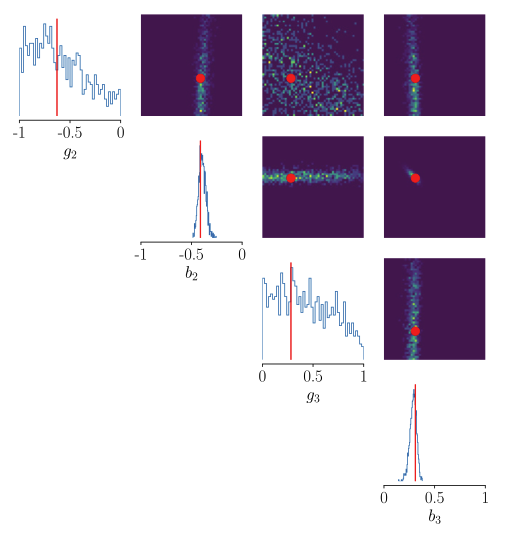
\includegraphics[width=0.92\linewidth]{figs/posterior_SPNE.png}
        \caption{\scriptsize SNPE posteriors on the \cite{brock_heterogeneous_1998} model; red lines mark the true posterior mean. Source: \cite{dyer_black-box_2024}.}
        \label{fig:snpe-posterior}
    \end{figure}
    \end{column}
    \end{columns}
\end{frame}



% =====================================================================
%  Application: CANVAS wage-price spiral (slides 9-17 of
%  presentation_short.tex from the wage-price-spiral paper repo)
% =====================================================================
\section{Application: CANVAS wage--price spiral}

\begin{frame}{Pricing mechanism}
    \begin{itemize}
        \item The CANVAS model uses the \textbf{expected marginal cost + markup rule}.
        \[ P_i(t) = MC^e_i(t)\cdot\mu_i(t) \]
        \item Marginal cost is determined by the sum of all production costs.
        \[ MC_i(t) =\underbrace{\frac{(1+\tau^{\text{SIF}}(t))\overline{w}_i(t)}{\overline{\alpha}_i(t)} P^{\text{W}}(t)}_{\text{unit labour costs}} + \underbrace{\frac{1}{\beta_i(t)}\sum_g a_{s g}(t) \bar{P}_g(t)}_{\text{unit intermediate costs}} + \underbrace{\frac{\delta_i(t)}{\kappa_i(t)} \bar{P}^{C F}(t)}_{\text{unit capital costs}}. \]
        \item Marginal costs are inflated by expected inflation.
        \[ MC^e_i(t) = (1 + \pi^e(t))\cdot MC_i(t-1). \]
        \item The markup is updated by demand pull (explained next slide).
        \[ \mu_i(t) = (1 + \pi^{DP}(t))\,\mu_i(t-1) \]
    \end{itemize}
\end{frame}

\begin{frame}{Demand pull mechanisms}
    \begin{columns}
        \begin{column}{0.55\textwidth}
            \begin{itemize}
                \item Firms form firm-level expectations using two indicators from the previous period: \textbf{excess supply} (difference between supply and realized demand) and their \textbf{price deviation} from competitors' average price.
                \item Based on these conditions, firms follow four strategic scenarios that determine whether to adjust price or production:\\
                a) clear inventory by decreasing prices, \\b) decrease production to match demand, \\c) capture profitable market opportunity, and \\d) increase prices to increase margins.
            \end{itemize}
        \end{column}
        \begin{column}{0.45\textwidth}
            \begin{figure}
                \centering
                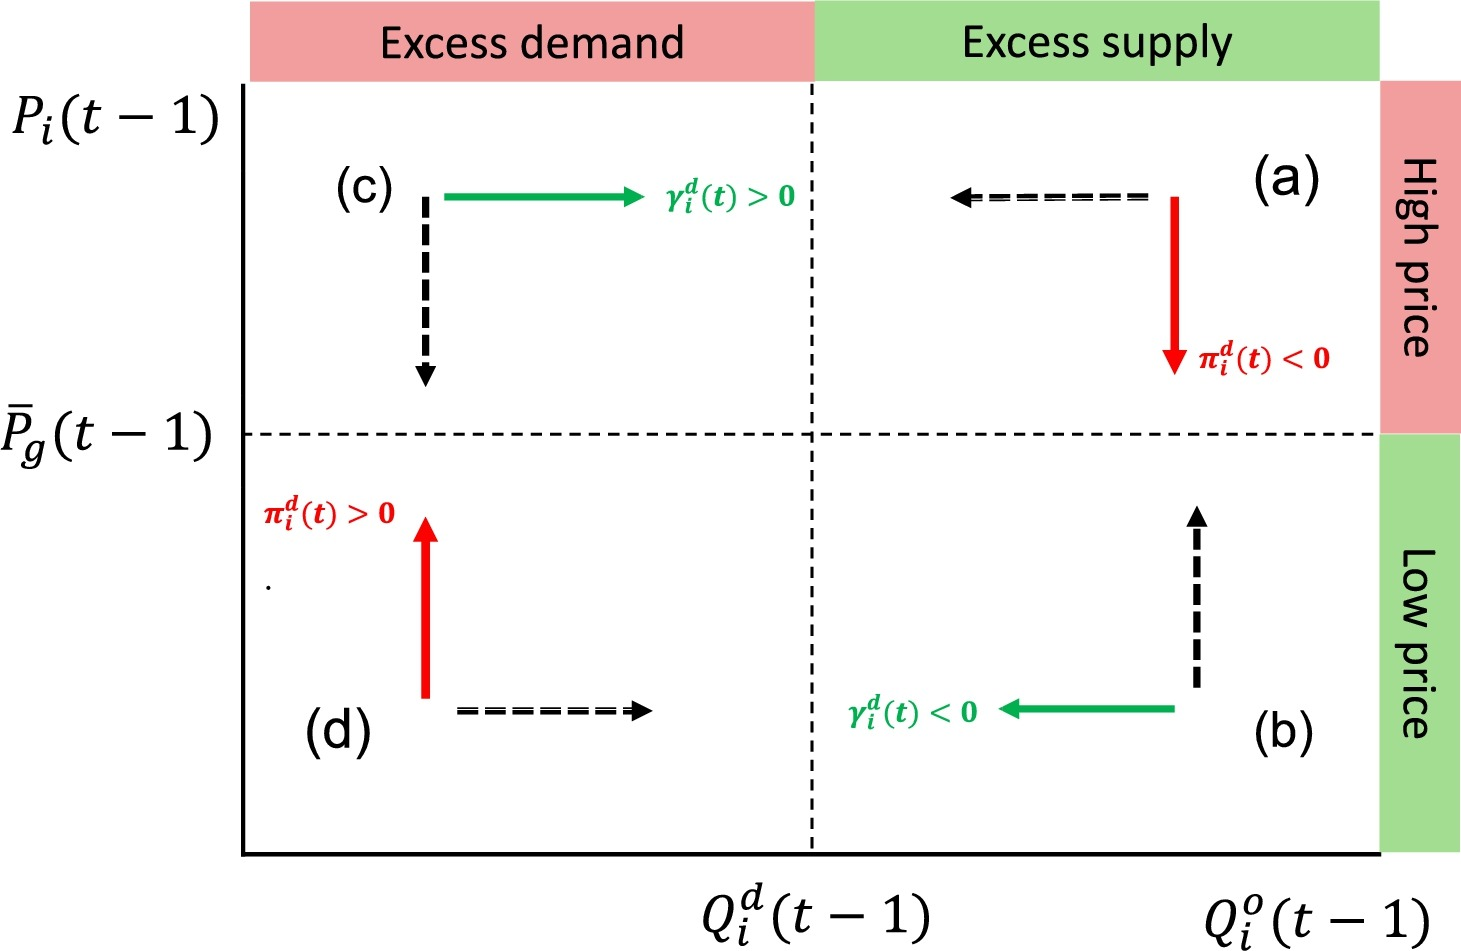
\includegraphics[width=\textwidth]{figs/wps_demand_pull}
                \caption{\scriptsize Source: \cite{hommes_canvas_2025}}
            \end{figure}
        \end{column}
    \end{columns}
\end{frame}

\begin{frame}{Demand pull mechanisms (formulae)}
    \begin{itemize}
        \item Demand pull inflation is determined by (scenario (a) and (d))
        \footnotesize
        \[ \pi_i^d(t)= \begin{cases}\dfrac{Q_i^d(t-1)}{Q_i^o(t-1)}-1 & \text{if } Q_i^o(t-1) \leq Q_i^d(t-1) \text{ and } P_i(t-1)<\bar{P}_g(t-1) \\ & \text{or if } Q_i^o(t-1)>Q_i^d(t-1) \text{ and } P_i(t-1) \geq \bar{P}_g(t-1) \\ 0 & \text{otherwise.}\end{cases} \]
        \item \normalsize Quantity setting is given by $Q_i^{\mathrm{s}}(t)=Q_i^{\mathrm{o}}(t-1)\left(1+\gamma^e(t)\right)\left(1+\gamma_i^d(t)\right)$, where $\gamma^e(t)$ is the aggregate growth rate and $\gamma_i^d(t)$ is idiosyncratic growth.
        \item $\gamma_i^d(t)$ is determined by (scenario (b) and (c))
        \footnotesize
        \[ \gamma_i^d(t)= \begin{cases}\dfrac{Q_i^d(t-1)}{Q_i^o(t-1)}-1 & \text{if } Q_i^o(t-1) \leq Q_i^d(t-1) \text{ and } P_i(t-1) \geq \bar{P}_g(t-1) \\ & \text{or if } Q_i^o(t-1)>Q_i^d(t-1) \text{ and } P_i(t-1)<\bar{P}_g(t-1) \\ 0 & \text{otherwise.}\end{cases} \]
    \end{itemize}
\end{frame}

\begin{frame}{CANVAS pricing mechanism implicit assumptions}
    \begin{itemize}
        \item The CANVAS pricing equation can be written as
        \[
        P_i(t)=P_i(t-1) \cdot \underbrace{\left(1+\phi^{DP}\pi_i^d(t)\right)}_{\substack{\text{Demand-pull}\\\text{inflation}}} \cdot \underbrace{\left(1+\phi^{CP}\pi_i^c(t)\right)}_{\substack{\text{Cost-push}\\\text{inflation}}} \cdot \underbrace{\left(1+\phi^{AE}\pi^e(t)\right)}_{\substack{\text{Aggregate}\\\text{inflation expectation}}}
        \]
        \item However, the CANVAS model implicitly assumes that $\phi^{DP}=\phi^{CP}=\phi^{AE}=1$.
        \item This assumes all inflation costs pass through to prices, but firms actually absorb some costs.
        \item Moreover, it assumes that wages are indexed fully and that the quantity demand-pull channel has 100\% strength.
    \end{itemize}
\end{frame}

\begin{frame}{Sectoral inflation decomposition: wage shock, non-estimated ABM}
    \begin{figure}
        \centering
        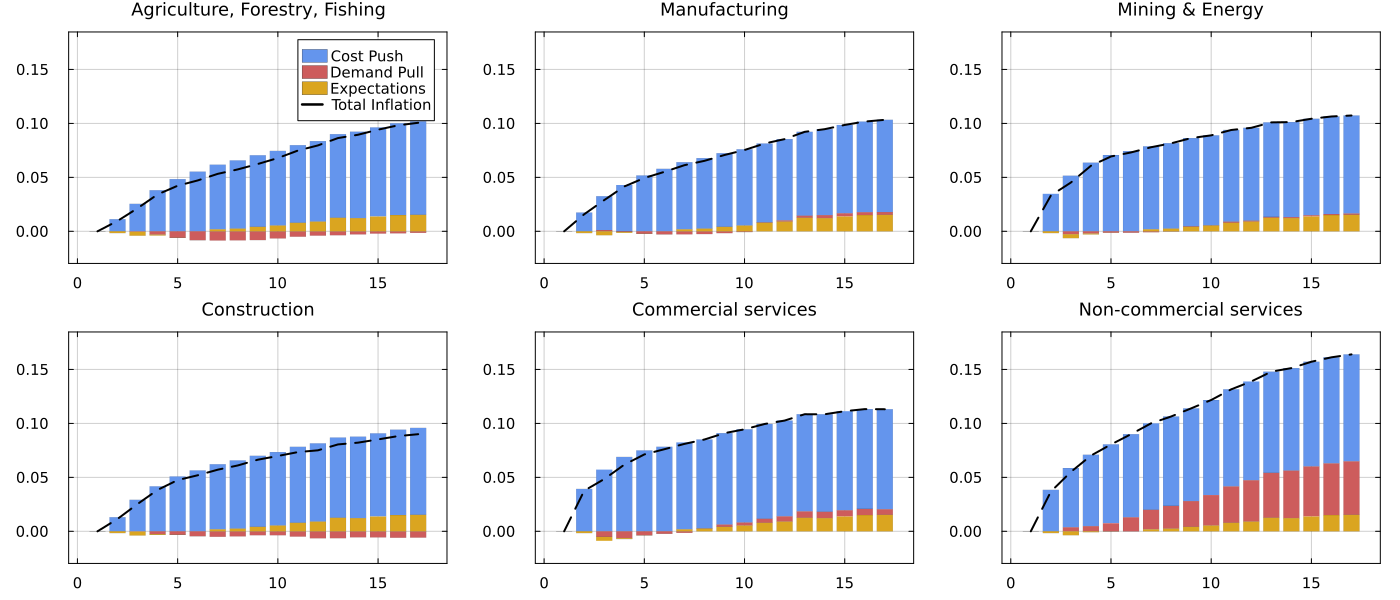
\includegraphics[width=.85\linewidth]{figs/wps_infl_decomp_no_estimate}
        \caption{\scriptsize Sectoral inflation decomposition following 10\% wage shock. Stacked bars show contributions from cost pass-through, demand pull, and expectations components. Dashed line indicates total cumulative inflation difference from baseline simulation over 16 quarters.}
    \end{figure}
\end{frame}

\begin{frame}{Sectoral inflation decomposition: wage shock, estimated ABM}
    \begin{figure}
        \centering
        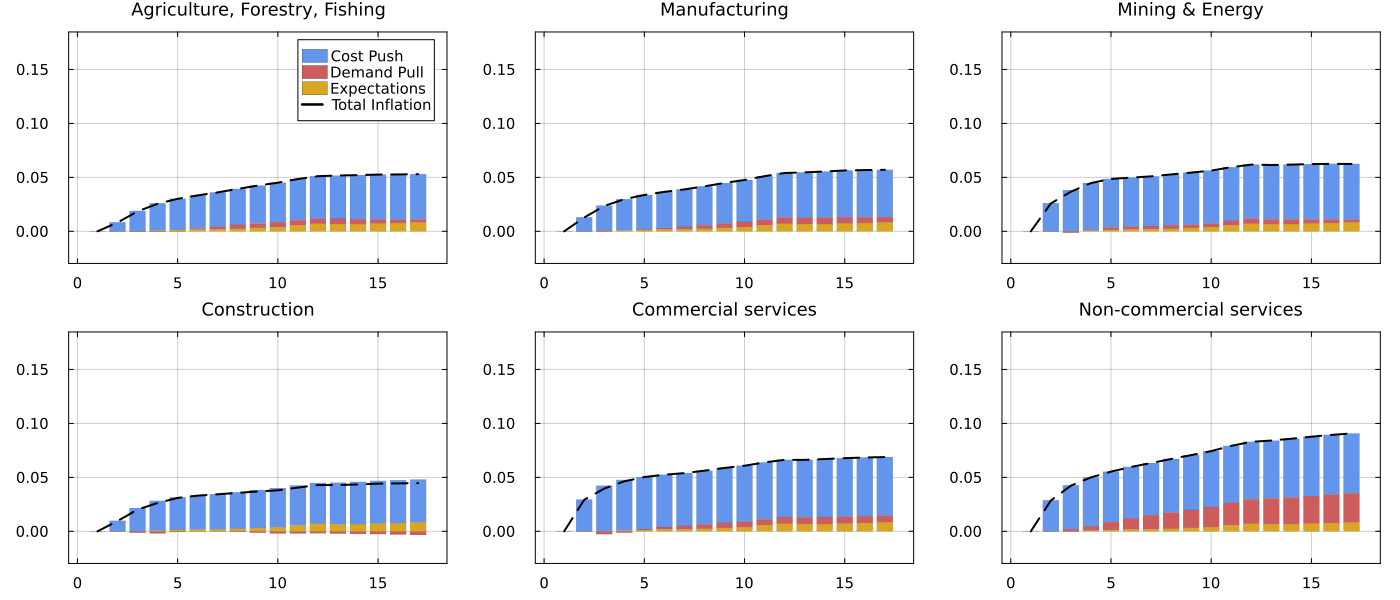
\includegraphics[width=.85\linewidth]{figs/wps_infl_decomp_estimated}
        \caption{\scriptsize Sectoral inflation decomposition following 10\% wage shock. Stacked bars show contributions from cost push, demand pull, and expectations inflation. Dashed line indicates total cumulative inflation difference from baseline simulation over 16 quarters.}
    \end{figure}
\end{frame}

\begin{frame}{Further sectoral inflation decomposition: non-estimated ABM}
    \begin{figure}
        \centering
        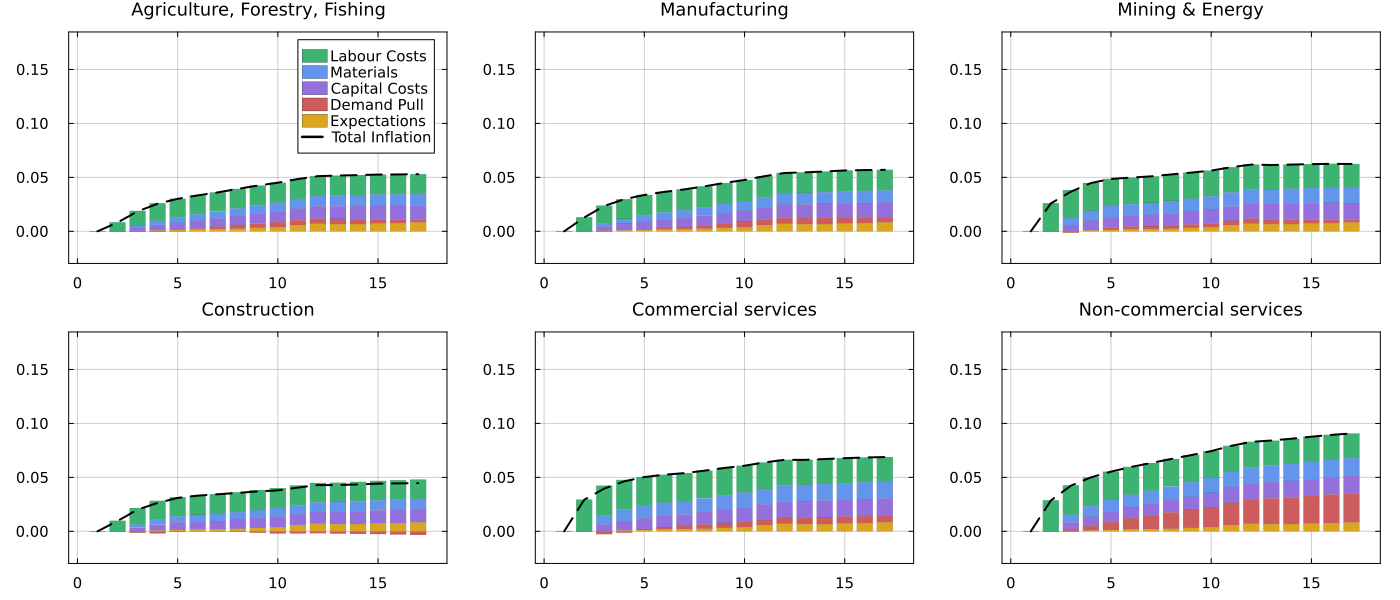
\includegraphics[width=.85\linewidth]{figs/wps_infl_decomp_components}
        \caption{\scriptsize Sectoral inflation decomposition following 10\% wage shock. Stacked bars show contributions from demand pull inflation, labour costs, intermediate products, capital costs, and aggregate inflation. Dashed line indicates total cumulative inflation difference from baseline simulation over 16 quarters.}
    \end{figure}
\end{frame}

\section{Discussion}

\begin{frame}{Concluding Remarks}
\begin{itemize}
    \item \textbf{Qualitative} macro ABMs (e.g.\ \cite{assenza_emergent_2015}) generate emergent business cycles, but are validated only against stylised facts.
    \item We have covered the \textbf{quantitative} agent-based model of \cite{poledna_economic_2019} and its calibration to Eurostat national-accounts data.
    \item We have covered \textbf{simulation-based Bayesian inference} for ABMs via neural posterior estimation \citep{dyer_black-box_2024}.
    \item We are now at the frontier of agent-based modelling!
\end{itemize}
\end{frame}

\begin{frame}
    \begin{center}
    {\Large Thank you very much for your attention!\\}
    \vspace{3cm}
  { \LARGE \textbf{Questions?}}
\end{center}
\end{frame}
    

\begin{frame}[allowframebreaks]{Bibliography}
    \bibliography{example}
\end{frame}


\appendix
\section{Firms}
\begin{frame}{Decentralized market}
\label{Firm}
\begin{itemize}
    \item  Each firm $i$ experiences demand $Q_{i, t}^d$ from consumers. Realized sales depend on production and inventory.
    \footnotesize
 \begin{equation} \displaystyle
Q_{i,t}^{\mathrm{d}} \begin{cases} \displaystyle <Y_{i,t}+S_{i,t-1} & \text { if demand from consumers is smaller than supply from firm } i, \text { and } \\ \displaystyle =Y_{i,t}+S_{i,t-1} & \text { if demand from consumers exactly matches supply from firm } i, \text { and } \\ \displaystyle >Y_{i,t}+S_{i,t-1} & \text { if demand from consumers is larger than supply from firm } i,\end{cases}
\end{equation}
\item  \normalsize Sales $Q_{i, t}$ are the realized demand dependent on the supply available from firm $i$ after the production process has taken place:
$$
Q_{i, t}=\min \left(S_{i, t-1}+Y_{i, t}, Q_{i, t}^d\right)
$$
\item   Matching probabilities depend on size of the firm and on the price \footnotesize \begin{equation} 
\begin{aligned}
p r _{i,t}^{\text {price }}  & =\frac{e^{-2 P _{i,t} }}{\sum_{i \in I_{s=g}} e^{-2 P _{i,t} }} \\
p r _{i,t}^{\text {size }}  & =\frac{Y _{i,t} }{\sum_{i \in I_{s=g}} Y _{i,t} } \\
p r _{i,t}^{\text {cum }}  & =\frac{p r _{i,t}^{\mathrm{price}} +p r _{i,t}^{\text {size }} }{2}
\end{aligned}
\end{equation}
\normalsize
\end{itemize}
        \hyperlink{ReturnOverview}{\beamerbutton{Return}}
\end{frame}
\begin{frame}{Quantity and Price Setting}


    \begin{itemize}
        \item Quantity setting is based on expected growth rates
        \begin{equation}
Q_{i,t}^s = Q_{i,t-1}^d(1+\gamma_t^{\mathrm{e}} ).
\end{equation} 
\item  Expectations are formed using AR(1) rule or VAR(1) rule
\item  Prices are determined the previous set price, expected inflation and the cost-structure of the firm: \footnotesize  $ 
P_{i,t}=P_{i,t-1} \cdot \underbrace{\left(1+\pi_{i,t}^c\right)}_{\begin{array}{c}
\text { Cost-Push } \\
\text { Inflation }
\end{array}} \cdot \underbrace{\left(1+\pi_t^e\right)}_{\begin{array}{c}
\text { Built-In } \\
\text { Inflation }
\end{array}},
$
\\ \normalsize where \footnotesize
\begin{equation}
 \pi_{i,t}^c=\underbrace{\frac{\left(1+\tau^{S I F}\right) \bar{w}_i}{\bar{\alpha}_i}\left(\frac{\bar{P}_t^{H H}}{P_{i,t}}-1\right)}_{\text {Increase of unit labour costs }}+\underbrace{\frac{1}{\beta_i}\left(\frac{\sum_g a_{s g} \bar{P}_{g,t-1}}{P_{i,t}}-1\right)}_{\text {Increase of unit material costs }}+\underbrace{\frac{\delta_i}{\kappa_i}\left(\frac{\bar{P}^{C F}_{t-1}}{P_{i,t}}-1\right)}_{\text {Increase of unit capital costs }} \forall i \in I_S .
\end{equation}
    \end{itemize}
    \normalsize
        \hyperlink{ReturnOverview}{\beamerbutton{Return}}

\end{frame}

\begin{frame}{External Finance}
    It is possible that firms need to finance current or future expenditures by borrowing.  Therefore, each firm forecasts future cash flow $\Delta D_{i,t}^{\mathrm{e}}$, which is equal to the expected change in deposits $D_{i,t}$:
\begin{equation}
    \scriptstyle \Delta D_{i,t}^{\mathrm{e}} =\underbrace{\Pi_{i,t}^{\mathrm{e}} }_{\text {Exp. profit }}-\underbrace{\theta L_{i,t-1} }_{\text {Deb instalment }}-\underbrace{\tau^{\mathrm{FIRM}} \max \left(0, \Pi_{i,t}^{\mathrm{e}} \right)}_{\text {Corporate taxes }}-\underbrace{\theta^{\mathrm{DIV}}\left(1-\tau^{\mathrm{FIRM}}\right) \max \left(0, \Pi_{i,t}^{\mathrm{e}} \right)}_{\text {Dividend payout }},
\end{equation}
    \hyperlink{ReturnOverview}{\beamerbutton{Return}}

\end{frame}
\begin{frame}{Profits}
    Firm profits $\Pi_{i,t}$ are an accounting measure.
\begin{equation}
\begin{aligned}
\Pi_{i,t}= & \underbrace{P_{i,t} Q_{i,t}}_{\text {Sales }}+\underbrace{P_{i,t} \Delta S_{i,t}}_{\text {Inventory change }}-\underbrace{\left(1+\tau^{\mathrm{SIF}}\right) w_{i,t} N_{i,t} \bar{P}_t^{\mathrm{HH}} }_{\text {Labour costs }} \\
& -\underbrace{\frac{1}{\beta_i} \bar{P}_{i,t} Y_{i,t}}_{\text {Material costs }}-\underbrace{\frac{\delta_i}{\kappa_i} P_{i,t}^{\mathrm{CF}}  Y_{i,t}}_{\text {Depreciation }}-\underbrace{\tau_i^{\mathrm{Y}} P_{i,t} Y_{i,t}-\tau_i^{\mathrm{K}} P_{i,t} Y_{i,t}}_{\text {Net taxes/subsidies on products/production}} \\
& -\underbrace{r_t \left(L_{i,t-1}+\max \left(0,-D_{i,t-1}\right)\right)}_{\text {Interest payments }}+\underbrace{\bar{r}_t  \max \left(0, D_{i,t-1}\right)}_{\text {Interest received }}
\end{aligned}
\end{equation}

 $r_t$ is the interest rate paid on outstanding loans.
     \hyperlink{ReturnOverview}{\beamerbutton{Return}}

\end{frame}
\begin{frame}{Cash Flow}
    Firm net cash flow is a measure how much liquidity is available for firms to use and is equal to changes in the deposit account:
\begin{equation}
\begin{aligned}
& \Delta D_{i,t}=\underbrace{P_{i,t} Q_{i,t}}_{\text {Sales }}-\underbrace{\left(1+\tau^{\mathrm{SIF}}\right) w_{i,t} N_{i,t} \bar{P}_t^{\mathrm{HH}}}_{\text {Labor costs }}-\underbrace{\bar{P}_{i,t} \Delta M_{i,t}}_{\text {Material costs }} \\
& -\underbrace{\tau_i^{\mathrm{Y}} P_{i,t} Y_{i,t}-\tau_i^{\mathrm{K}} P_{i,t} Y_{i,t}}_{\text {Net taxes/subsidies on products and production }}-\underbrace{\tau^{\mathrm{FIRM}} \max \left(0, \Pi_{i,t}\right)}_{\text {Corporate tax payments }} \\
& -\underbrace{\theta^{\mathrm{DIV}}\left(1-\tau^{\mathrm{FIRM}}\right) \max \left(0, \Pi_{i,t}\right)}_{\text {Dividend payments }}-\underbrace{r\left(L_{i,t-1}+\max \left(0,-D_{i,t-1}\right)\right)}_{\text {Interest payments }} \\
& +\underbrace{\bar{r}_t \max \left(0, D_{i,t-1}\right)}_{\text {Interest received }}-\underbrace{P_{i,t}^{\mathrm{CF}} I_{i,t}}_{\text {Investment costs }}+\underbrace{\Delta L_{i,t}}_{\text {New credit }}-\underbrace{\theta L_{i,t-1}}_{\text {Debt instalment }} . \\
&
\end{aligned}
\end{equation}
    \hyperlink{ReturnOverview}{\beamerbutton{Return}}

\end{frame}
\begin{frame}{More Accounting and Insolvency}
\begin{itemize}
    \item Firm deposits are equal to deposits plus net cash flow:
\begin{equation}
    D_{i,t}=D_{i,t-1}+\Delta D_{i,t}
\end{equation}
\item Debt follows the following law of motion:
\begin{equation}
    L_{i,t}=(1-\theta) L_{i,t-1}+\Delta L_{i,t}
\end{equation}
\item Firm equity $E_{i,t}$ is computed as a balancing item 
\begin{equation}
    E_{i,t}=D_{i,t}+\sum_g a_{s g} \bar{P}_{g,t} M_{i,t}+P_{i,t} S_{i,t}+\bar{P}^{\mathrm{CF}}_t  K_{i,t}-L_{i,t} \quad \forall i \in I_s
\end{equation}
\item When a firm has negative balance on their deposit account (cash flow insolvent, i.e. $D_{i,t}<0$) and has negative equity value (balance sheet insolvent, i.e. $E_{i,t}<0$), they become insolvent.
\end{itemize}
    \hyperlink{ReturnOverview}{\beamerbutton{Return}}
\end{frame}


\section{Government}
\begin{frame}{Government Overview}
\label{Government}

    \begin{itemize}
        \item Government purchases consumption on goods market
        \item Government levies taxes and takes social security contributions
        \item Government pays out social transfers
    \end{itemize}
       \hyperlink{ReturnOverview}{\beamerbutton{Return}}

\end{frame}
\begin{frame}{Government Revenue}
    Taxes, social contributions and other transfers from all sectors form the revenue of the government:
    \small
\begin{equation}
\begin{aligned}
& Y^{\mathrm{G}}_t=\underbrace{\left(\tau^{\mathrm{SIF}}+\tau^{\mathrm{SIW}}\right) \bar{P}^{\mathrm{HH}}_t\sum_{h \in H^{\mathrm{E}}_t} w_{h,t}}_{\text {Social security contributions }}+\underbrace{\tau^{\mathrm{INC}}\left(1-\tau^{\mathrm{SIW}}\right) \bar{P}^{\mathrm{HH}}_t \sum_{h \in H^{\mathrm{E}}_t} w_{h,t}}_{\text {Labor income taxes }} \\
& +\underbrace{\tau_h^{\mathrm{VAT}} \sum_h C_{h,t}}_{\text {Value added taxes }}+\underbrace{\tau^{\mathrm{INC}}\left(1-\tau^{\mathrm{FIRM}}\right) \theta^{\mathrm{DIV}}\left(\sum_i \max \left(0, \Pi_{i,t}\right)+\max \left(0, \Pi_{k,t}\right)\right)}_{\text {Capital income taxes }} \\
& +\underbrace{\tau^{\mathrm{FIRM}}\left(\sum_i \max \left(0, \Pi_{i,t}\right)+\max \left(0, \Pi_{k,t}\right)\right)}_{\text {Corporate income taxes }}+\underbrace{\tau^{\mathrm{CF}} \sum_h I_{h,t}}_{\text {Taxes on capital formation }} \\
& +\underbrace{\sum_i \tau_i^{\mathrm{Y}} P_{i,t} Y_{i,t}}_{\text {Net taxes/subsidies on products }}+\underbrace{\sum_i \tau_i^{\mathrm{K}} P_{i,t} Y_{i,t}}_{\text {Net taxes/subsidies on production }}+\underbrace{\tau_l^{\text {EXPORT }} \sum_l C_{l,t}}_{\text {Export taxes }} . \\
&
\end{aligned}
\end{equation}
\normalsize
    \hyperlink{ReturnOverview}{\beamerbutton{Return}}
\end{frame}

\begin{frame}{Government Deficit and Debt}
The government deficit (or surplus) is an accounting identity consisting of expenditures minus revenues:
\begin{equation}
\begin{aligned}
\scriptscriptstyle \Pi^{\mathrm{G}}_t= & \underbrace{\sum_{h \in H^{\text {inact }}} \bar{P}^{\mathrm{HH}}_t s b^{\text {inact }}_t+\sum_{h \in H^{\mathrm{U}}_t} \bar{P}^{\mathrm{HH}}_t \theta^{\mathrm{UB}} w_{h,t}+\sum_h \bar{P}^{\mathrm{HH}}_t s b_t^{\text {other }}}_{\text {Social benefits and transfers }} \\
& +\underbrace{\sum_j C^{\mathrm{G}}_{j,t}}_{\text {Government consumption }}+\underbrace{r^{\mathrm{G}} L_{t-1}^{\mathrm{G}}}_{\text {Interest payments }}-\underbrace{Y_t^{\mathrm{G}}}_{\text {Government revenues }} .
\end{aligned}
\end{equation}

The government debt is previous period government debt plus the current deficit:
\begin{equation}
    L^{\mathrm{G}}_t=L^{\mathrm{G}}_{t-1}+\Pi^{\mathrm{G}}_t.
\end{equation}
    \hyperlink{ReturnOverview}{\beamerbutton{Return}}
\end{frame}
\section{Banking Sector}
\begin{frame}{Banking Sector}
\label{Bank}

\begin{itemize}
    \item The bank provides loans to firms according to a risk assessment and a minimum capital requirement.
    \item The bank has to form expectations to be able to do so.
    \item The bank also holds deposits or provides credit to households.
    \item The bank receives interest payments and also needs to pay interest payments.
\end{itemize}
    \hyperlink{ReturnOverview}{\beamerbutton{Return}}

\end{frame}
\begin{frame}{Bank loan provision}

    The bank has to adhere to a minimum capital requirement coefficient $0<\zeta<1$:
\begin{equation}
\frac{E_{k,t}^{\mathrm{e}}}{\sum_{i=1}^I\left(L_{i,t}^{\mathrm{e}}+\Delta L_{i,t}\right)}=\frac{E_{k,t-1}}{\sum_{i=1}^I\left((1-\theta) L_{i,t-1}+\Delta L_{i,t}\right)} \geq \zeta,
\end{equation}
Due to fundamental uncertainty, the bank has to form expectations on the value of firm $i$ 's capital stock $\left(K_i^{\mathrm{e}}(t)\right)$ :
\begin{equation}
\frac{L_{i,t}^{\mathrm{e}}+\Delta L_{i,t}}{K_{i,t}^{\mathrm{e}}}=\underbrace{\frac{\overbrace{(1-\theta) L_{i,t-1}}^{=L_{i,t}^{\mathrm{e}}}+\Delta L_{i,t}}{\bar{P}^{\mathrm{CF}}_{t-1}\left(1+\pi_t^{\mathrm{e}}\right) K_{i,t-1}}}_{=K_{i,t}^{\mathrm{e}}} \leq \zeta^{\mathrm{LTV}} .
\end{equation}
      \hyperlink{ReturnOverview}{\beamerbutton{Return}}
\end{frame}
\begin{frame}{Bank Profits}
    The difference between interest revenues from loans provisions and costs due to interest payments on deposits held with the bank by firms and households are the bank's profits. 
\begin{equation}
    \begin{aligned}
\Pi_{k,t}= & \underbrace{r_t\left(\sum_{i=1}^I \left(L_{i,t-1}+\max \left(0,-D_{i,t-1}\right)\right)+\sum_{h=1}^H \max \left(0,-D_{h,t-1}\right)\right)+\bar{r}_t \max \left(0, D_{k,t-1}\right)}_{\text {Interest received }} \\
& -\underbrace{\bar{r}_t \sum_{i=1}^I \max \left(0, D_{i,t-1}\right)-\bar{r}_t \sum_{h=1}^H \max \left(0, D_{h,t-1}\right)-\bar{r}_t \max \left(0,-D_{k,t-1}\right)}_{\text {Interest payments }}
\end{aligned}
\end{equation}
The bank pays policy rate $\bar{r}_t$ on deposits.   The effective interest rate $r_t$ faced for bank credit or overdrafting is determined by the policy rate $\bar{r}_t$ and a fixed markup $\mu$ :
\begin{equation}
    r_t=\bar{r}_t+\mu
\end{equation}
\hyperlink{ReturnOverview}{\beamerbutton{Return}}

\end{frame}
\begin{frame}{Bank Accounting}
Bank equity is an accounting identity which is determined by bank profits or losses and is given by
    \begin{equation}
    \begin{aligned}
E_{k,t}= & E_{k,t-1}+\Pi_{k,t}-\underbrace{\theta^{\text {DIV }}\left(1-\tau^{\mathrm{FIRM}}\right) \max \left(0, \Pi_{k,t}\right)}_{\text {Dividend payments }} \\
& -\underbrace{\tau^{\mathrm{FIRM}} \max \left(0, \Pi_{k,t}\right)}_{\text {Corporate taxes }}-\underbrace{\sum_{i \in I^{\prime}}\left(L_{i,t}-D_{i,t}-\zeta^{\mathrm{b}} \bar{P}_i^{\mathrm{CF}}(t) K_{i,t}\right)}_{\text {Write-off of bad debt }},
\end{aligned}
\end{equation}
      \hyperlink{ReturnOverview}{\beamerbutton{Return}}

\end{frame}
\section{Central Bank}
\begin{frame}{Central Bank}
\label{CentralBank}
    \begin{itemize}
        \item Central bank sets policy rate according to Taylor rule.
        \item The central bank receives revenues from interest payments on government debt.
        \item The central bank receives or pays interest depending on the net position of the advances or reserves to the banking system.
        \item The central bank balance sheet determines whether the economy is a net creditor or net debtor to the rest of the world.
    \end{itemize}
    \hyperlink{ReturnOverview}{\beamerbutton{Return}}

\end{frame}
\begin{frame}{Interest Rate Setting}
    A generalized Taylor rule \citep{taylor_discretion_1993} determines the policy rate. We use the same rule as \cite{blattner_towards_2010}, which includes a "growth" rule specification: 
\begin{equation}
    \bar{r}_t=\rho \bar{r}_{t-1}+(1-\rho)\left(r^*+\pi^*+\xi^\pi\left(\pi^{\mathrm{EA}}_t-\pi^*\right)+\xi^\gamma \gamma^{\mathrm{EA}}_t\right)
\end{equation}
where $\rho$ is a measure for gradual adjustment of the policy rate, $r^*$ is the real equilibrium interest rate, $\pi^*$ is the inflation target of the central bank, $ \xi^\pi$ is the weight the central bank puts on inflation targeting and $\xi^\gamma$ the weight placed on economic growth, respectively. 
\hyperlink{ReturnOverview}{\beamerbutton{Return}}

\end{frame}
\begin{frame}{Central Bank Accounting}
    The difference between revenues from interest payments on government debt, as well as revenues or costs  is defined as the central bank's profits.
\begin{equation}
    \Pi^{\mathrm{CB}}_t=r^{\mathrm{G}} L^{\mathrm{G}}_{t-1}-\bar{r}_t D_{k,t-1} .
\end{equation}
The central bank's equity $E^{\mathrm{CB}}_t$ in an accounting identity dependent on its profits or losses and its past equity. 
\begin{equation}
    E^{\mathrm{CB}}_t=E^{\mathrm{CB}}_{t-1}+\Pi^{\mathrm{CB}}_t .
\end{equation}
\hyperlink{ReturnOverview}{\beamerbutton{Return}}

\end{frame}
\begin{frame}{Central Bank Accounting}
    The following law of motion determines the net creditor/debtor position of the national economy to the rest of the world $\left(D^{\mathrm{RoW}}_t\right)$:
\begin{equation}
    D^{\mathrm{Row}}_t=D^{\mathrm{RoW}}_{t-1}-\underbrace{\left(1+\tau^{\mathrm{EXPORT}}\right) \sum_l C_{l,t}}_{\text {Exports }}+\underbrace{\sum_m P_{m,t} Q_{m,t}}_{\text {Imports }} .
\end{equation}
This connects the change in the amount of deposits in the banking system to the government deficit (surplus)  and to the balance of trade: 
\begin{equation}
    \begin{aligned}
E^{\mathrm{CB}}_t+D^{\mathrm{RoW}}_t & =L^{\mathrm{G}}(t)-D_{k,t} \\
& =L^{\mathrm{G}}_t-\sum_{i=1}^I D_{i,t}-\sum_{h=1}^H D_{h,t}-E_{k,t}+\sum_{i=1}^I L_{i,t} .
\end{aligned}
\end{equation}
\hyperlink{ReturnOverview}{\beamerbutton{Return}}
\end{frame}
\section{Rest of The World}
\begin{frame}{Rest of the World}
\label{Imports}
    \begin{itemize}
        \item Supply of imports and and demand of exports are determined by an AR(1) processes.
        \item Demand for imports and supply of exports are endogenous.
        \item Realized imports and exports are determined by the search-and-matching mechanism.
    \end{itemize}
    \hyperlink{ReturnOverview}{\beamerbutton{Extensive description}}
\end{frame}
\begin{frame}{Imports}
    \begin{itemize}
        \item Total supply of Imports $Y^I_t$ in real terms follows an AR(1) rule.
        \item Thus the $m$-th, $(m\in\{1, \ldots, S\})$, foreign firm representing an industry $s$ imports the principal product $g$: $    Y_{m,t}=c_{g=s}^I Y^{\mathrm{I}}_t.$
        \item  Import price is assumed to develop similarly as the average sectoral domestic adjusted for expected inflation: $P_{m,t}=\overline{P}_{g,t-1} (1+\pi^e_t)$.
        \item Sales of imports are equal to the realized demand which is an outcome of the search-and-matching process on the goods markets: $Q_{m,t}=\min \left(Y_{m,t}, Q_{m,t}^d\right)$.
    \end{itemize}
                    \hyperlink{ReturnOverview}{\beamerbutton{Return}}
\end{frame}
\begin{frame}{Exports}
    \begin{itemize}
        \item Total demand for export is $C^E_t$ is assumed to be exogenous and follows an AR(1) rule.
        \item  The total demand for exports is uniformly distributed to $L$ foreign consumers and attributed to goods $g$ :
\begin{equation}
    C_{l,t}^{\mathrm{d}}=\frac{C^{\mathrm{E}}_t \sum_g c_{g,t}^{\mathrm{E}} \bar{P}_{g,t-1}\left(1+\pi^{\mathrm{e}}_t\right)}{L},
\end{equation}
\item The demand for exported goods by the $l$-th foreign consumer to purchase the $g$-th good is given by
\begin{equation}
    C_{l g,t}^{\mathrm{d}}=\frac{c_g^{\mathrm{E}} \bar{P}_{g,t-1}}{\sum_g c_g^{\mathrm{E}} \bar{P}_{g,t-1}} C_{l,t}^{\mathrm{d}}.
\end{equation}
\item Realized consumption by foreign consumers is again determined by the search-and-matching process on goods
markets.
    \end{itemize}
                    \hyperlink{ReturnOverview}{\beamerbutton{Extensive description}}
\end{frame}


\end{document}
